\documentclass[times, utf8, diplomski]{fer}
\usepackage{booktabs}
\usepackage{graphicx}
\usepackage{subcaption}
\usepackage{algorithm}
\usepackage{algorithmic}
\usepackage{amsmath}
\usepackage{hyperref}

\graphicspath{{Assets/}}

\begin{document}

\thesisnumber{2633}
\title{Kartezijsko genetsko programiranje u konvoluciji slike}
\author{Lukas Šestić}

\maketitle

% Ispis stranice s napomenom o umetanju izvornika rada. Uklonite naredbu \izvornik ako želite izbaciti tu stranicu.
\izvornik

% Dodavanje zahvale ili prazne stranice. Ako ne želite dodati zahvalu, naredbu ostavite radi prazne stranice.
\zahvala{}

\tableofcontents

\chapter{Uvod}
Prva asocijacija na spomen napredne obrade slike je umjetna inteligencija i duboke neuronske mreže.
Uz to, tehnika konvolucije pokazala se daleko najprimjerenija za rješavanje problema. \\
Problem koji se javlja s rezultantnim modelima dubokih neuronskih mreža je što su gotovo uvijek nerazumljivi i rade kao \emph{crne kutije}.
Točnije, ljudima je teško razumjeti i objasniti kako je mreža došla do izlaza kojeg je stvorila. \\
Velika prednost modela nastalim genetskim algoritmom je razumljivost. \\
Genetsko programiranje se i ranije koristilo kao način obrade slike uz razlike kao što su (\cite{cgp_image_processing}):
\begin{itemize}
	\item jednostavnija arhitektura, npr. stablo
	\item manji skup funkcija
\end{itemize}

Ovaj rad baviti će se uporabom \emph{Kartezijskog genetskog programiranja} (\emph{CGP}), čija je arhitektura inspirirana dubokim neuronskim mrežama, u svrhu obrade i analize slike. \\
U nastavku rada, ukratko će se objasniti što je genetsko programiranje te kako radi.
Detaljno će se predstaviti \emph{CGP} kao tehnika genetskog programiranja, izraziti prednosti nad klasičnim metodama te predstaviti način na koji su implementirane konvolucijske tehnike u svrhu provedbe eksperimenata.
Predstaviti će se svi provedeni eksperimenti, prikazati će se i objasniti rezultati te usporediti s željenim.
Na kraju, okušati će se u korištenju \emph{CGP-a} kao metode izrade \emph{autoencoder-a} te će se ispitati ograničenja korištenja genetskog programiranja kao prikladne tehnike za generiranje uzoraka zadane raspodjele.

Cilj rada je dati čitatelju ideju o radu i performansama \emph{CGP-a} kroz provedene eksperimente te poslužiti kao inspiracija i početka točka za buduće eksperimente.


\chapter{Genetsko programiranje}
\section{Genetsko programiranje}
\emph{Genetsko programiranje} (\emph{GP}) je evolucijski algoritam koji do rješenja dolazi iterativno mjenjajući populaciju sve dok uvjet zaustavljanja nije zadovoljen (\cite{conv_gen_programming}).

Inspiraciju vuče iz prirode.
Algoritam počinje s nasumično nastalom populacijom koja se poboljšava kroz ograničen broj generacija.
Nastanak svake generacije započinje izborom jedinki (detaljno opisane u nastavku).
Izbor nije nasumičan niti determinističan, boljim jedinkama daje se prednost pri izboru no i one lošije mogu biti izabrane.
Nedeterminističnost izbora rezultira širem pretraživanju prostora rješenja, ne ograničenim samo na najbolje jedinke.
Iz jedinki nastaju nove kao rezultat genetskih operatora \emph{Križanja} i \emph{Mutacije}.
Ciklus se ponavlja sve dok jedna od dvije stvari nije zadovoljena:
\begin{itemize}
	\item{Dosegnut najveći broj iteracija ili evaluacija}
	\item{Postignuta željena preciznost rješenja (npr. $greska \leq 10^{-3}$})
\end{itemize}
Na kraju postupka, dobiveni model osim što se može koristiti u željenu svrhu, lako se može izučiti i interpretirati, jer za razliku od neuronskih mreža, način na koji ulaz postaje izlaz jasno je čitljiv. \\
Jednostavan primjer genetskog algoritma vidljiv je u pseudokodu ~\ref{alg:gp_example}

\begin{algorithm}
	\caption{Jednostavni genetski algoritam (\cite{wong2015evolutionary})}
	\label{alg:gp_example}
	\begin{algorithmic}
		\STATE $P(t)$: Roditeljska populacija u generaciji $t$
		\STATE $O(t)$: Populacija potomaka u generaciji $t$
		\STATE $P(t)=$ stvori\_pocetnu\_populaciju()
		\WHILE{uvjet zaustavljanja nije zadovoljen}
			\STATE $P^{'}(t) =$ izabrani roditelji iz $P(t)$
			\STATE $O(t + 1) =$ potomci nastali krizanjem jedinki iz $P^{'}(t)$
			\STATE $O(t + 1) = mutiraj\ O(t + 1)$
			\STATE $evaluiraj(O(t + 1))$
			\STATE $P(t + 1) = O(t + 1)$
			\STATE $t = t + 1$
		\ENDWHILE
	\end{algorithmic}
\end{algorithm}

\subsection{Jedinka populacije}
Jedinka populacije u genetskom algoritmu predstavlja jedno moguće rješenje na problem koji smo postavili.
Svaka jedinka je definirana s dvije stavke:
\begin{itemize}
	\item{Genotipom}
	\item{Načinom mapiranja genotipa u \emph{fenotip}}
\end{itemize}
Na najnižoj razini, svaka jedinka je jedan genotip. 
U praksi, genotip može biti prikazan na bilo koji način koji odgovara korisniku algoritma, no neke od najčešćih struktura su vektori brojeva, simbola ili bitova, fiksne ili varijabilne duljine, te stablaste strukture (\cite{naturally_selecting_algorithms}).
Korisnik koji koristi \emph{genetski algoritam} (GA) za pronalazak rješenja mora također definirati mapiranje $genotip \rightarrow fenotip$.
Genotipom možemo smatrati ono što koristi algoritam kako bi stvorio fenotip, dok je fenotip jedno od mogućih rješenja na problem koji rješavamo.
Što to znači?
Ukoliko je zadatak GA iz skupa točaka provesti simboličku regresiju $A\sin(Bx + C)$ gdje su $A$, $B$ i $C$ nepoznate varijable genotip bi se mogao prikazati kao vektor s broja s pomičnim zarezom.
Dalje, pravilo mapiranja genotipa u fenotip bi moglo biti da element na prvom mjestu odgovara vrijednosti koju pridajemo varijabli $A$ i tako dalje za varijable $B$ i $C$ (~\ref{fig:genotype_phenotype_map}).
Također, bitno je kvantificirati kvalitetu jedinke.
Ta mjera najčešće se naziva kondicija (\emph{eng. fitness}).
Sve jedinke populacije dobivaju kondiciju na temelju istog pravila kako bi bili međusobno usporedivi.
Jedinka s najvećom kondicijom smatra se najkvalitetnijom i najboljim rješenjem na problem koji se rješava.

\begin{figure}
	\caption{Mogućnosti spremanja i korištenja genotipa tijekom izvođenja genetskog algoritma}
	\begin{subfigure}[t]{0.45\textwidth}
		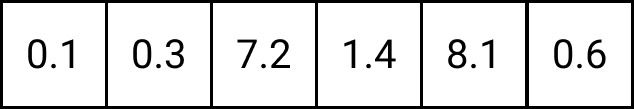
\includegraphics[width=\textwidth]{Illustrations/float_genotype.png}
		\caption{Genotip prikazan brojem s pomičnim zarezom}
	\end{subfigure}
	\hspace{\fill}
	\begin{subfigure}[t]{0.45\textwidth}
		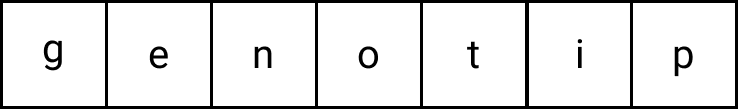
\includegraphics[width=\textwidth]{Illustrations/char_genotype.png}
		\caption{Genotip prikazan ascii znakovima}
	\end{subfigure}
	\label{fig:genotype_types}
\end{figure}

\begin{figure}
	\centering
	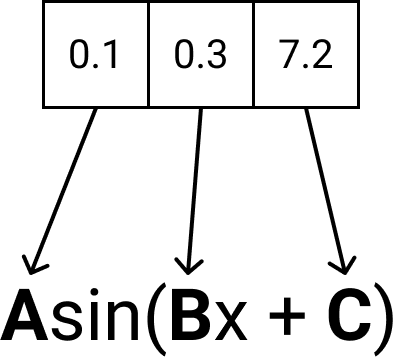
\includegraphics[width=0.4\linewidth]{Illustrations/genotype_phenotype_mapping.png}
	\caption{Primjer mapiranja genotipa u fenotip}
	\label{fig:genotype_phenotype_map}
\end{figure}

\subsection{Genetski operatori}
Genetski operatori pružaju osnovni mehanizam pretrage genetskog algoritma.
Za zadatak imaju stvarati nova rješenja uz efektivnu pretragu prostora rješenja.
Izvode se na primitivu jedinki, genotipu, te se nerjetko međusobno izvode u kombinaciji jer samostalno nisu uvijek efektivni.
U nastavku su opisane 2 osnovne vrste genetskih operatora, križanje i mutacija.

\subsubsection{Križanje}
Operator križanja u genetskom algoritmu oponaša reprodukciju u biološkom svijetu.
Od dvije jedinke stvara nove primjenjujući neko definirano pravilo kombinacije njihovih genotipa.
Križanje nije trivijalno kao na prvi pogled, te je usko ovisno o izboru strukture podataka s kojom definiramo genotip (~\cite{wong2015evolutionary}). \\
Na slici ~\ref{fig:crossover} prikazan je primjer jednog od operatora križanja koje ću detaljnije opisati u nastavku.

\begin{figure}
	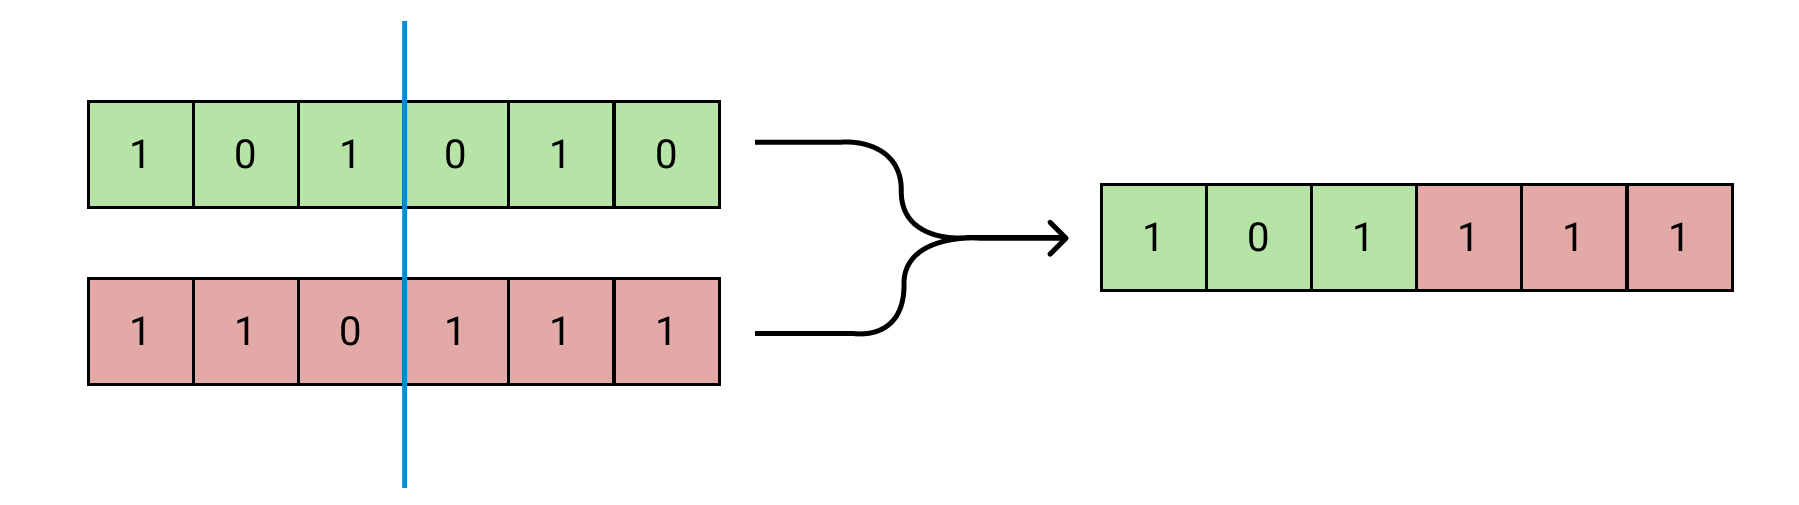
\includegraphics[width=\linewidth]{Illustrations/crossover.png}
	\caption{Jednostavni primjer rezultata primjene operatora križanja}
	\label{fig:crossover}
\end{figure}

\paragraph{Križanje u k točaka}
se koristi tako da se odabere $k$ nasumičnih točaka koje služe kao granica između kojih se uzimaju dijelovi dva različita genotipa.
Često se odabere $k = 1$ (primjer na slici ~\ref{fig:crossover}) zbog svoje jednostavnosti.
Ono što se često zamjera križanju u jednoj točki je pristranost poziciji genotipa.
To znači da će pri odabiru dva roditeljska genotipa $P_1$ i $P_2$ lijevi dio novonastalog genotipa uvijek pripasti pripadajućem dijelu $P_1$ a desni $P_2$.
Rješenje na taj problem, osim odabira $k > 1$, je stvaranje dva potomka koja se zatim evaluiraju, nakon čega se potomak koji se pokaže boljim prenosi u sljedeću generaciju populacije (ilustracija ~\ref{fig:position_bias}).

\begin{figure}
	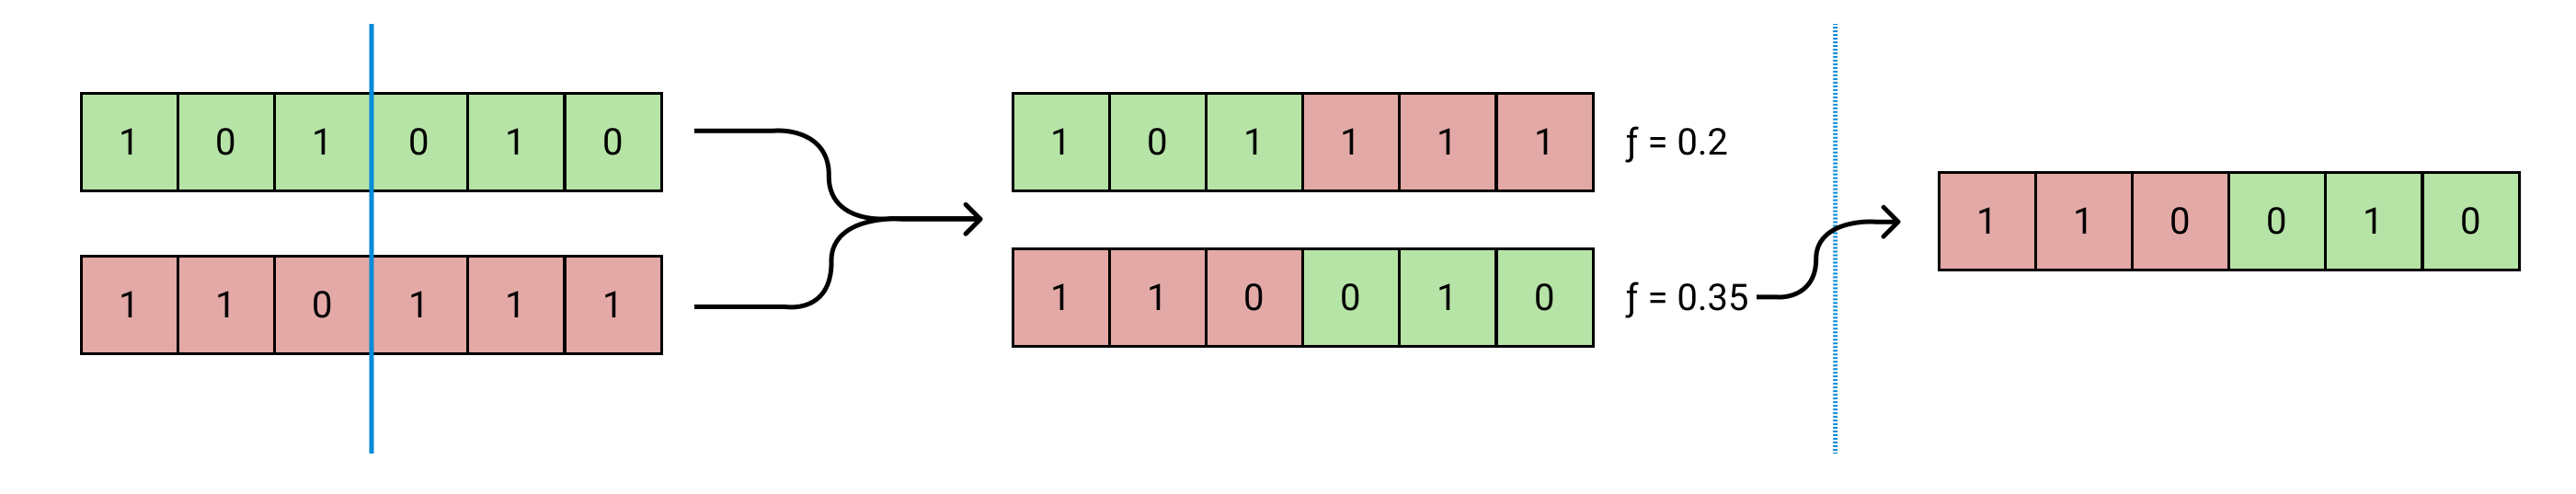
\includegraphics[width=\linewidth]{Illustrations/position_bias.png}
	\caption{Primjer rješavanja problema pristranosti pozicije}
	\label{fig:position_bias}
\end{figure}

\paragraph{Ujednačeno križanje (\emph{eng. Uniform crossover})}
tretira svaki gen u genotipu zasebno što osigurava da svaki roditeljski gen ima jednaku vjerojatnost da se prenese na novonastali genotip.
Postupak se može definirati kao:
\[
	O[n] = \left\{\begin{array}{lr}
			P_1[n], & \text{za } 0 \leq \alpha \leq 0.5 \\
			P_2[n] & \text{za } 0.5 < \alpha \leq 1
		\end{array}\right\}
\]
Također, grafički prikazano na ilustraciji ~\ref{fig:uniform_crossover}.

\begin{figure}
	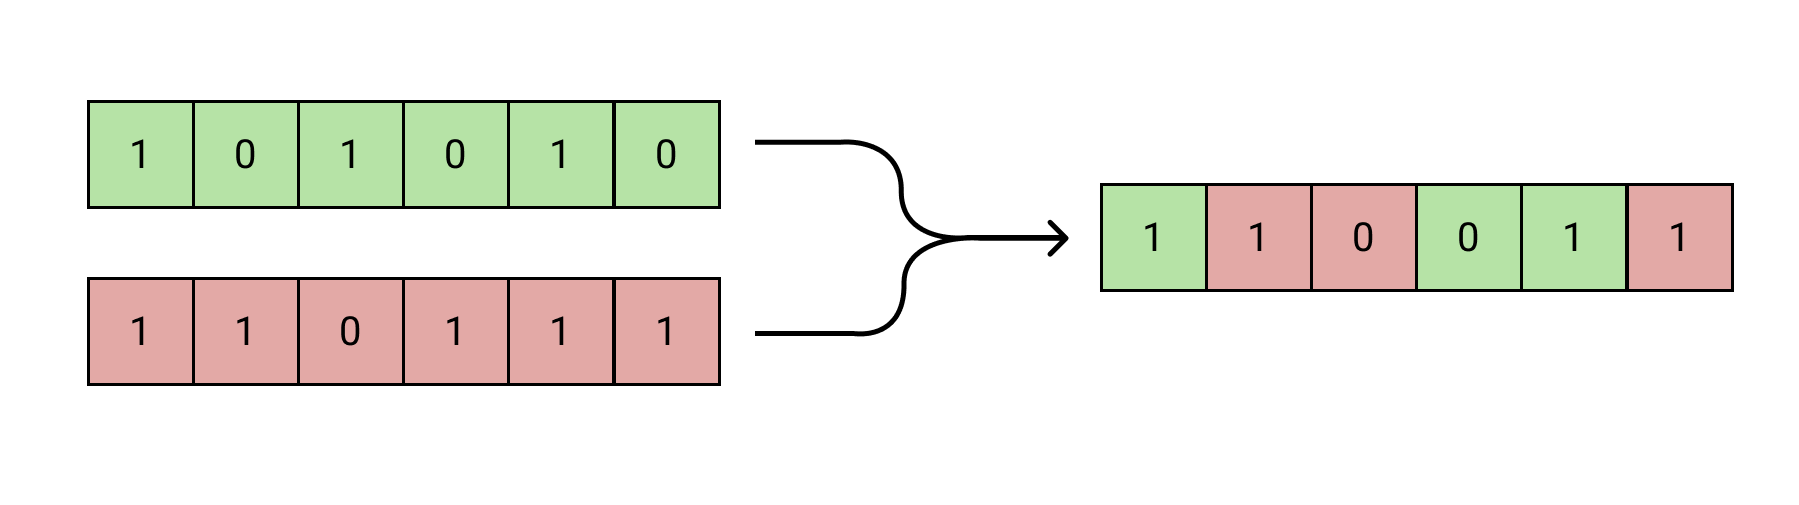
\includegraphics[width=\linewidth]{Illustrations/uniform_crossover.png}
	\caption{Rezultat primjene ujednačenog križanja}
	\label{fig:uniform_crossover}
\end{figure}

\subsubsection{Mutacija}
Analogno istoimenoj pojavi u biološkom svijetu, mutacija unosi male i nasumične promjene u genotip.
Primjena mutacije na genotip ne mora nužno promjeniti ni jedan gen, a može promjeniti i svaki.
Šansa za mutaciju se zadaje od strane korisnika i ne treba biti prevelika jer, u tom slučaju algoritam se svodi na nasumičnu pretragu.
U najviše slučajeva, vrijednost mutacije $\leq 5\%$ daje dobre rezultate.
Isto tako, vrijednost mutacije ne mora biti statična kroz cijeli algoritam.
Primjerice, u ranim iteracijama algoritma može biti korisno imati nešto veću vjerojatnost za mutaciju kako bi pretraživali veći prostor rješenja a u kasnijim iteracijama, kada smo nešto bliže rješenju, smanjiti tu vjerojatnost kako bismo manjim izmjenama došli do globalnog optimuma.
Razlog zbog kojeg se koristi mutacija je što pridonosi različitosti u populaciji.
Korištenje samo križanja potiče problem konvergencije u lokalnom minimumu, što se pokušava izbjeći unošenjem nasumičnih promjena tako potičući razliku između jedinki.
Imajući to na umu važno je napomenuti da se genetski algoritam može koristiti koristeći samo mutaciju.
Isto se ne može reći za križanje.
Pri rješavanju problema, ne moramo se ograničiti na jednu vrstu mutacije već se dodatna nasumičnost može unjeti korištenjem više vrsta mutacije odjednom.

\paragraph{Okretanje bitova (\emph{eng. Bit flip})} 
je mutacija koja je primjenjiva samo na genotipima opisanim kao vektor bitova \emph{npr.} $[1 0 0 1 0 1 1 0 1 1 1]$.
Uz zadani parametar $\alpha$, koji primjerice može biti $\alpha = \frac{1}{duljina\ vektora}$, svaki bit uz zadanu vjerojatnost negira, pretvarajući $0 \rightarrow 1$ i suprotno (ilustracija ~\ref{fig:bit_flip_mutation}).

\begin{figure}
	\centering
	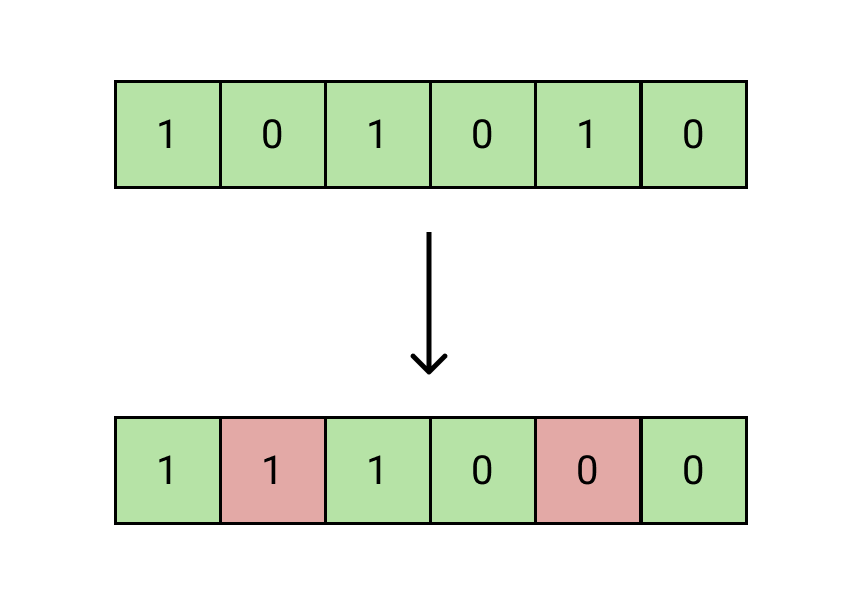
\includegraphics[width=0.5\linewidth]{Illustrations/bit_flip_mutation.png}
	\caption{Rezultat primjene mutacije okretanjem bitova}
	\label{fig:bit_flip_mutation}
\end{figure}

\paragraph{Ujednačeno mutiranje (\emph{eng. Uniform mutation})}
se koristi na genotipima opisanim cijelim brojevima ili brojevima s pomičnom točkom.
Svaki gen koji mutira mijenja u novu nasumičnu vrijednost unutar dozvoljene domene ukoliko ona postoji (ilustracija ~\ref{fig:uniform_mutation}).

\begin{figure}
	\centering
	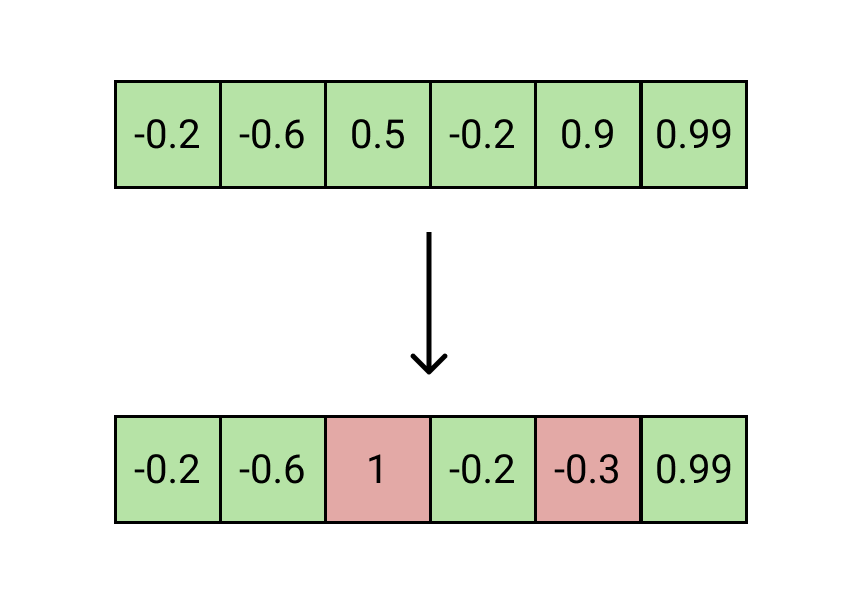
\includegraphics[width=0.5\linewidth]{Illustrations/uniform_mutation.png}
	\caption{Rezultat primjene ujednačene mutacije na genotip za čije gene vrijedi $gen \in [-1, 1]$}
	\label{fig:uniform_mutation}
\end{figure}

\paragraph{Mutiranje Gaussovim šumom}
osim nasumične varijable $\alpha$ koja predstavlja vjerojatnost da će gen biti mutiran, koristi i nasumičnu varijablu $X$, distribuiranu Gaussovom raspodjelom, odnosno $X \sim \mathcal{N}(\mu,\sigma^2)$ gdje $\mu$ srednja vrijednost, a $\sigma^2$ varijanca.
Svakom genu koji će biti mutiran pridodaje se šum $X$ (ilustracija ~\ref{fig:gaussian_mutation}).

\begin{figure}
	\centering
	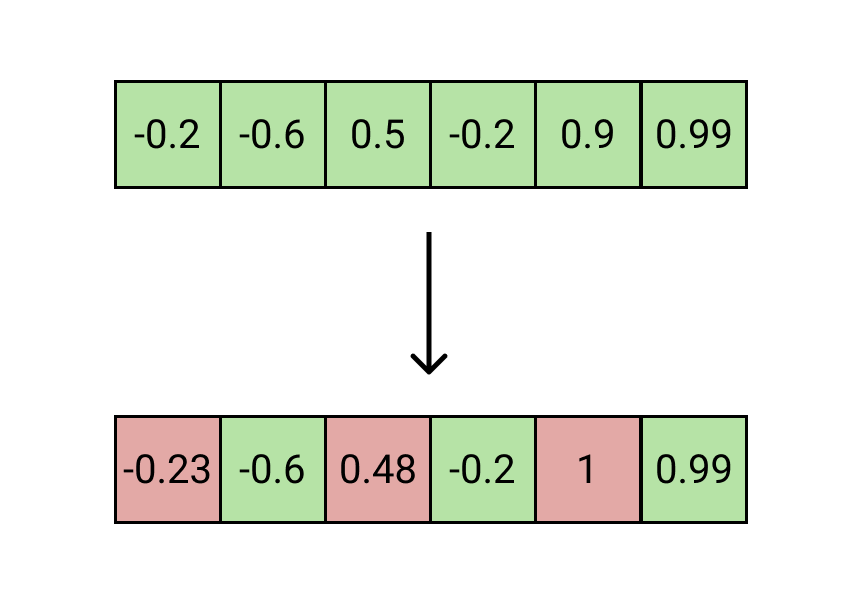
\includegraphics[width=0.5\linewidth]{Illustrations/gaussian_mutation.png}
	\caption{Rezultat primjene mutacije Gaussovim šumom}
	\label{fig:gaussian_mutation}
\end{figure}

\subsection{Elitizam}
Elitizam je broj najboljih jedinki koje se bez mutiranja prenose u sljedeću generaciju, osiguravajući preživljavanje najboljih jedinki (~\cite{elitism}).
Definira se cjelobrojnom vrijednosti $\in [0, broj\ jedinki\ u\ populaciji]$.
U slučaju da je vrijenost 0, ni jedna jedinka se ne prenosi.
Pretpostavka iza korištenja elitizma je da će nastati dobar balans između različitosti populacije uzrokovane križanjem i mutacijom potičući pretraživanje širokog prostora rješenja i konstantnog globalnog napretka uzrokovanog elitizmom.
Rezultat pretpostavke je brža i monotonija konvergencija ka globalnom optimumu.
Graf ~\ref{fig:elitism} prikazuje utjecaj elitizma pri optimizaciji strategije usmjeravanja podataka prenošenim bežičnom mrežom.

\begin{figure}
	\centering
	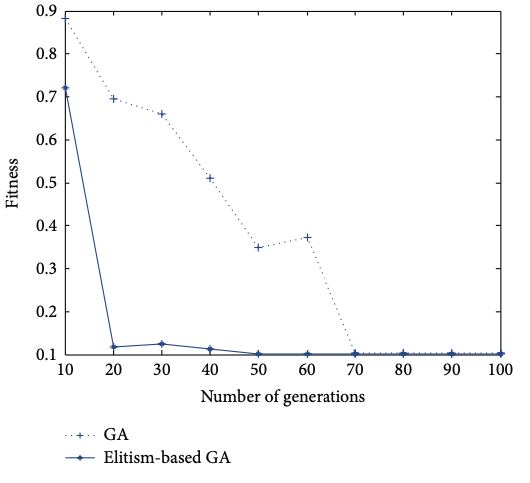
\includegraphics[width=0.7\linewidth]{SourcedGraphs/elitism_comparison.png}
	\caption{Usporedba izvođenja genetskog algoritma sa i bez elitizma pri rješavanju optimizacijskog problema}
	\label{fig:elitism}
\end{figure}


\subsection{Uvjet zaustavljanja}
Genetski algoritmi su posebno prikladni i efikasni u rješavanje problema s velikim prostorima pretrage te problemima gdje uobičajeni algoritmi ne bi bili polinomijalno učinkoviti (npr. NP-potpuni problemi) (~\cite{brassard1988algorithmics}).
Pripadanje u skupinu \emph{mekog računarstva} ne garantira potpuno precizna rješenja, već dovoljno precizna za samouvjereno donošenje zaključaka na kraju izvođenja.
Također, algoritam se izvodi kroz ograničeni broj koraka.
Postavlja se pitanje, kada zaustaviti koračanje, odnosno algoritam?
U praksi, najčešće se koriste sljedeća tri uvjeta zaustavljanja (~\cite{ga_stopping_criteria}):
\begin{itemize}
	\item Dosegnut najveći dozvoljeni broj generacija
	\item Dosegnut najveći dozvoljeni broj evaluacija kondicijske funkcije
	\item Dosegnuta željena preciznost
\end{itemize}
Ograničenje najvećeg dozvoljenog broja generacija i evaluacija kondicijske funkcije su statička ograničenja.
Je li uopće moguće precizno odrediti najbolje vrijednosti za statička ograničenja? \\
Slijepo postavljanje abnormalno velikih vrijednosti te postepeno smanjivanje kroz sljedeća pokretanja algoritma je iznimno neučinkovito.
Potrebno je određeno znanje o problemu kako bi se postavila barem približno precizna ograničenja na duljinu pretrage prostora rješenja. \\
Dosegnuta željena preciznost je dinamičko ograničenje koje se može i ne mora doseći u bilo kojem trenutku.
To znači da za neki problem, za koji smo postavili ograničenje na npr. najviše $100$ generacija, možemo doseći uvjet zaustavljanja npr. grešku $\leq 10^{-3}$ već nakon desetak generacija ako je problem jednostavan ili smo slučajno dobili početnu točku blisku globalnom optimumu.
Analogno tome, zapinjanje u lokalnom optimumu može izazvati istek statičkih ograničenja bez postizanja željene preciznosti. \\
Znači li spomenuto da je dostizanje željene preciznosti najbolje mjerilo kvalitete dobivenog modela? \\
U kontekstu \emph{strojnog učenja}, čemu pripada i genetsko programiranje, često se spominju različiti skupovi podataka. \\
Razlikujemo tri skupa (~\cite{datasets}):

\paragraph{Skup za trening}
su podaci na temelju kojih se model \emph{uči} uspoređujući svoje izlaze sa željenim iz skupa.

\paragraph{Skup za validaciju} 
je objektivniji skup podataka na kojima se model nikad ne uči.
S obzirom na svojstvo učenja da će pokušati najbolje preslikati ulaze na izlaze što sličnije željenim iz skupa za trening lako može doći do \emph{pretreniranja}.
S tim na umu, validacijski skup je objektivnije mjerilo kvalitete modela.

\paragraph{Testni skup}
su podaci koji se prezentiraju konačnom modelu.
Odvajaju se od cjelokupnog skupa podataka na samom početku eksperimenta te su rezervirani za konačne modele koji se žele daljnije ispitati.
Imitiraju podatke i situacije iz stvarnog svijeta jer kako su podaci odvojeni na samom početku, model ih nikad nije vidio.
Slično validacijskom skupu s razlikom da se u ni jednoj točki postupka treniranja podaci iz testnog skupa ne prikažu modelu. \\

Spomenuti skupovi se nadovezuju na svojstvo algoritma da će kroz vrijeme samo preciznije svoje izlaze približavati onima na kojima se trenira dosežući pritom fazu pretreniranja.
Graf ~\ref{fig:train_test_loss} prikazuje ovisnost odstupanja na različitim skupovima podataka te optimalnu točku s najboljim objektivnim modelom.
Područje lijevo od označenog trenutka je vrijeme tijekom kojeg je model uz stalno učenje bio objektivan. 
Desno od trenutka je nastupilo pretreniranje.
Model sve bolje preslikava ulaze onima iz skupa za trening, no sve ostalo postaje nepreciznije.
Graf ~\ref{fig:overfitting} Prikazuje rad objektivnog i pretreniranog modela.

\begin{figure}
	\caption{Grafički prikaz odstupanja kroz iteracije na trening i validacijskom skupu podataka te prikaz rada pretreniranog modela}
	\begin{subfigure}[t]{0.48\textwidth}
		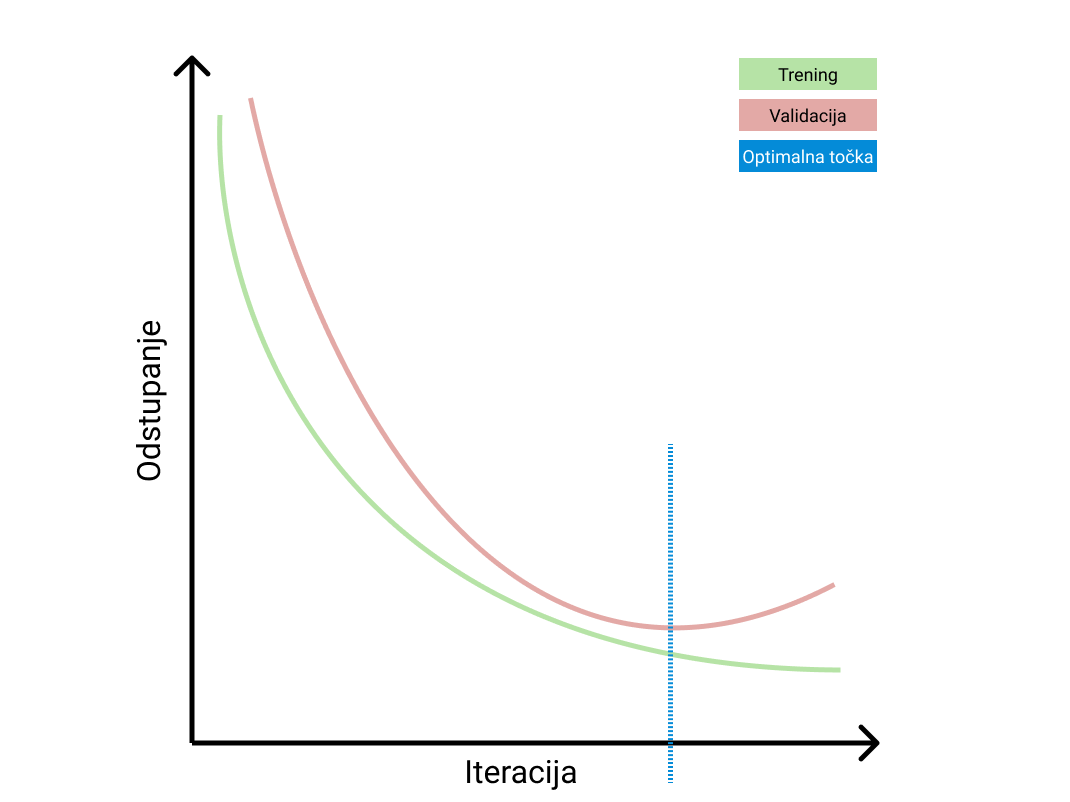
\includegraphics[width=\textwidth]{Illustrations/train_test_loss.png}
		\caption{Odstupanje na različitim skupovima podataka kroz iteracije}
		\label{fig:train_test_loss}
	\end{subfigure}
	\hspace{\fill}
	\begin{subfigure}[t]{0.48\textwidth}
		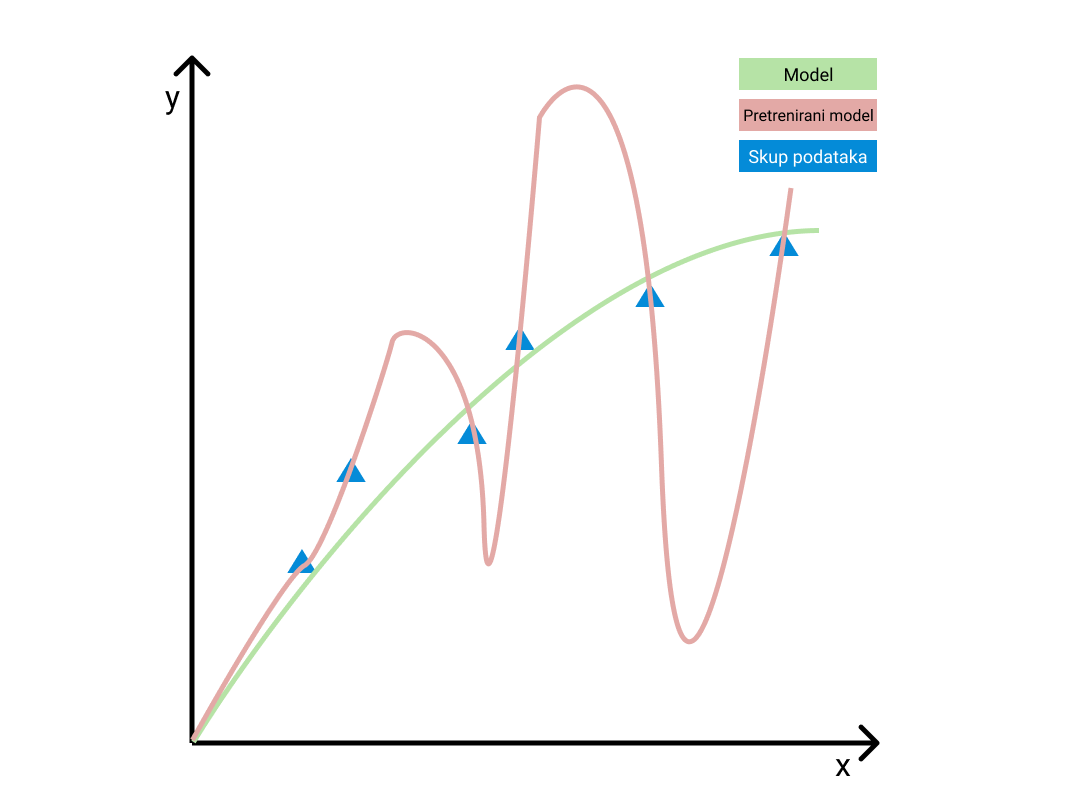
\includegraphics[width=\textwidth]{Illustrations/overtraining.png}
		\caption{Rad objektivnog i pretreniranog modela}
		\label{fig:overfitting}
	\end{subfigure}
\end{figure}

Iz priloženog je vidljivo kako tema uvjeta zaustavljanja nije jednostavna kao što se na prvu čini te postoji puno parametara koji uvjetuju koji model uzeti.
~\cite{ga_stopping_criteria} naglašava da korištenje isključivo statičkih ograničenja ne garantira dobre rezultate.
Dinamička provjera sa drugim skupovima podataka je pouzdana i provjerena metoda uz manu što znatno utječe na vrijeme izvođenja algoritma.
~\cite{fuzzy_logic} ispituju i predlažu korištenje meke logike kako bi definirali uvjet zaustavljanja.
Samo pogađanje i pretpostavka dobrih parametara je iznimno kompliciran problem koji se pojavljuje i prije pokretanja samog eksperimenta.
Također, s obzirom na rast računalne moći i na trenutne trendove (~\cite{ga_stopping_criteria}), adaptivni i dinamički uvjeti zaustavljanja su višestruko isplativi za korištenje tijekom rješavanja problema.

\section{Kartezijsko genetsko programiranje}
Kartezijsko genetsko programiranje (\emph{CGP}) nije ništa drugo nego arhitektura prikazivanja jedinki tijekom izvođenja algoritma. 
Mnoštvo benefita koje nosi sa sobom čine CGP iznimno fleksibilnim i prikladnim za rješavanje problema u kojima bismo inače posegnuli za arhitekturom sintaksnog stabla ili čak neuronskom mrežom.

\subsection{Genotip}
Jezgra CGP jedinke su čvorovi (\emph{eng. nodes}).
Genotip je vektor cjelih brojeva (gena) fiksne duljine gdje svaki ne preklapajuči podskup služi kao opisnik jednog čvora.
Razlikujemo dvije vrste gena.

\paragraph{Funkcijski gen}
definira adresu funkcije koju čvor izvodi na izlazu.
Adrese funkcije pohranjene su u tablici funkcija (npr. tablica \ref{table:function_table}), definirane od strane korisnika.

\begin{table}
	\centering
	\begin{tabular}{||c c||}
		\hline
		Adresa funkcije & Funkcija \\ [0.5ex]
		\hline\hline
		0 & $x \times y$ \\
		1 & $x + y$ \\
		2 & $\frac{x}{y}$ \\
		3 & $\sin{x}$ \\
		4 & $\cos{x}$ \\ 
		5 & $max(x, y)$ \\
		6 & $min(x, y)$ \\ [1ex]
		\hline
	\end{tabular}
	\caption{Primjer funkcijske tablice}
	\label{table:function_table}
\end{table}

\paragraph{Vezni gen (\emph{eng. Connection gene})}
definira izvor podataka za čvor.
Indeksiran je jednakim pravilom kao i čvorovi jer čvor kao ulaz prima vrijednost čvora sloja plićeg od sebe ili direktno iz ulaza u graf. \\
\\
Osim opisa skrivenih čvorova (čvorova između ulaza i izlaza), genotip na kraju sadrži i $n_o$ (broj izlaza) veznih gena. \\
Primjer genotipa vidljiv je na ilustraciji \ref{fig:genotype}

\begin{figure}
	\centering
	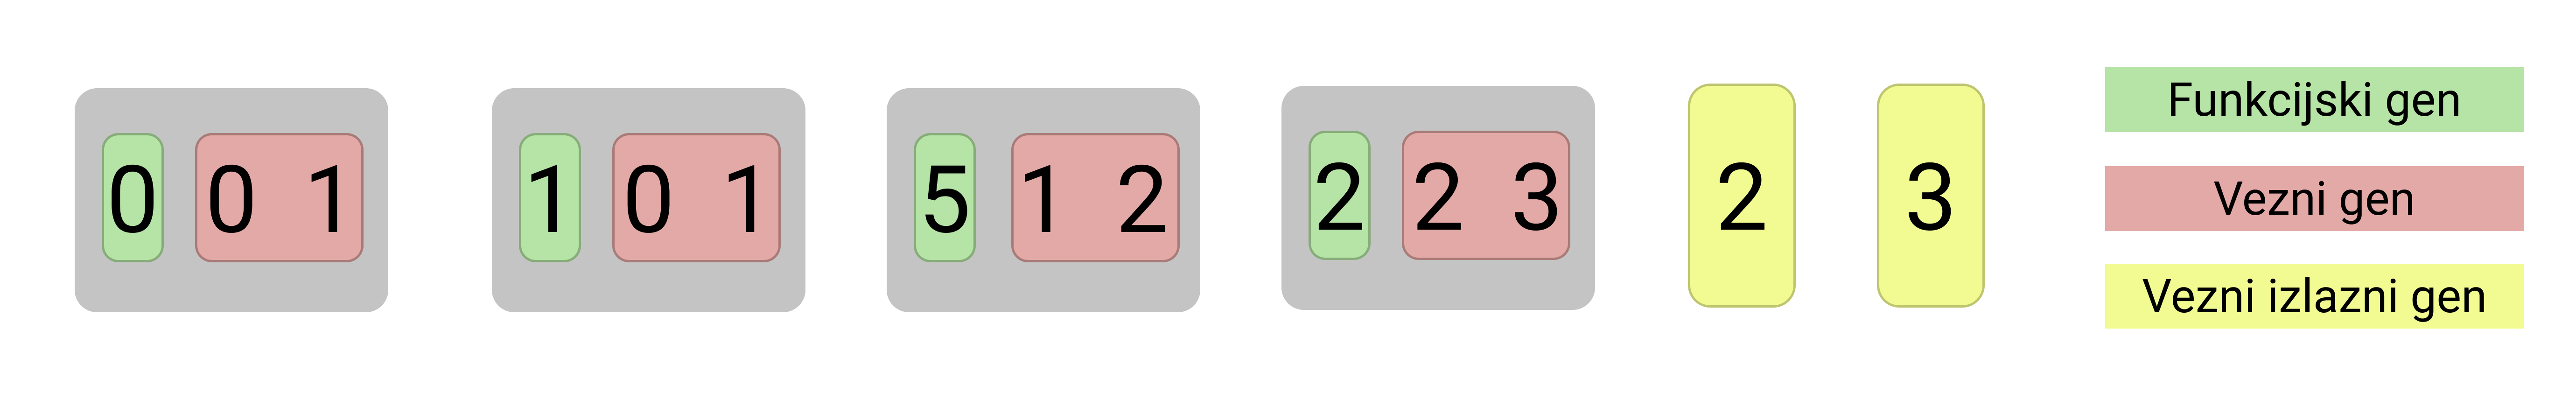
\includegraphics[width=\linewidth]{Illustrations/genotype.png}
	\caption{Primjer genotipa za CGP s dva ulaza, četiri sakrivena čvora i dva izlaza}
	\label{fig:genotype}
\end{figure}

\subsection{Arhitektura}
% Aciklički graf, dvodimenzionalnost, veličina, levelsback, nektivni čvor i kako utječe na fenotip
CGP jedinke prikazane su u obliku usmjerenih acikličnih grafova u dvodimenzionalnom prostoru (\cite{cgp}).
Arhitektura CGP jedinke definirana je sljedećim vrijednostima:
\begin{itemize}
	\item Broj ulaza $n_i$
	\item Broj izlaza $n_o$
	\item Broj skrivenih redaka i stupaca $n_r$ i $n_c$
	\item Broj najvećih vrijednost unazad koje čvor može uzimati (\emph{eng. levelsback}) $l$
\end{itemize}
Broj izlaza $>1$ nije tipična stvar za genetsko programiranje i veliki je benefit korištenja arhitekture inspirirane neuronskom mrežom.
Brojem najvećih vrijednosti unazad koje može čvor primiti definiramo složenost modela.
Priroda grafa takva je da se vrijednosti od prvog stupca šalju dublje sve do izlaza.
Ako je $l = 1$ definirali smo da svaki čvor može biti spojen najpliće u sloj prije sebe.
Tu mu dajemo manje slobode te ga ograničavamo na složenije modele, nego da smo dozvolili $l > 1$.
Naravno, ako želimo dozvoliti spajanje s čvorom iz bilo kojeg stupca, postavljamo  $l=n_c$.

Parametrima $n_r$ i $n_c$ definiramo broj računalnih čvorova kao $L_n = n_r \times n_c$.
Imajući to na umu, ne moraju svi čvorovi biti iskorišteni.
Čvorove koji ne vode prema izlazu nazivamo ne-aktivnim (\emph{eng. non-coding}).
Njihovi ulazi i funkcija nemaju nikakav utjecaj na konačni izlaz iz mreže.
Tu je vidljiva razlika između genotipa koji ima fiksnu i konstantnu duljinu i fenotipa čija duljina i oblik ovise o aktivnim i neaktivnim čvorovima.
Na slici \ref{fig:cgp_gene_feno} vidljiv je genotip CGP mreže i pripadajući fenotip s jasno označenim ne-aktivnim čvorovima i pravilima indeksiranja.

\begin{figure}
	\centering
	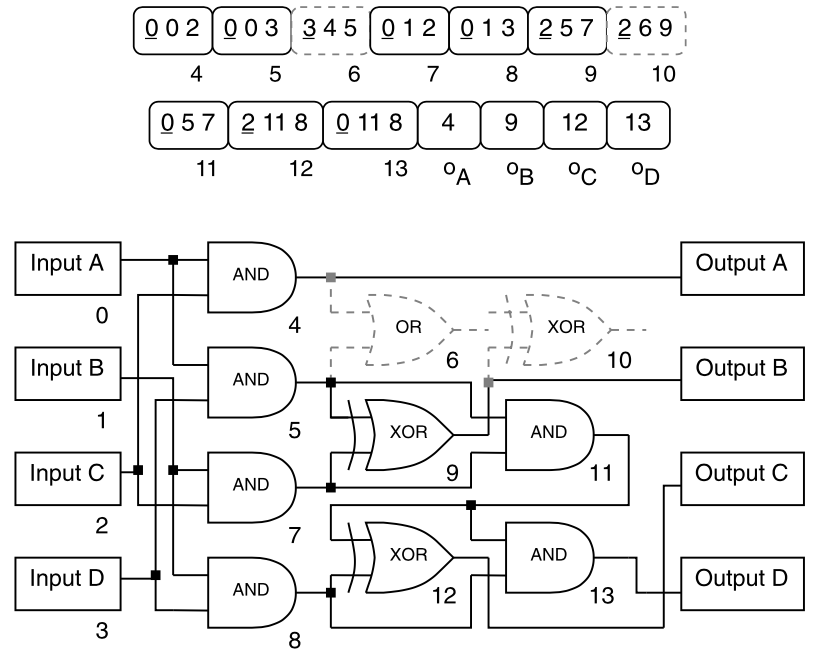
\includegraphics[width=\linewidth]{Illustrations/inactive_nodes.png}
	\caption{CGP genotip i fenotip digitalnog kruga. U čvorovima su vidljive funkcije koje izvode, a čvorovi koji su iscrtani su neaktivni jer ne vode ni na jedan izlaz. Također vidljivi su indeksi svakog čvora i u genotipu i fenotipu. Izvor \cite{cgp}}
	\label{fig:cgp_gene_feno}
\end{figure}

I u praksi i u tablici \ref{table:function_table} vidljivo je da nemaju sve funkcije jednak broj ulaza.
Na primjer, funkcija pod rednim brojem $4$, odnosno $\cos{x}$, ima jedan ulaz, dok funkcija $5$, $max(x, y)$ ima dva ulaza.
Treba li svakom čvoru dati točno onaj broj ulaza koliko traži njegova funkcija?
Naravno da ne, svako mutiranje mreže zahtjevalo bi ažuriranje broja ulaza u čvor i unijelo dodatnu kompleksnost u izvođenje te bi narušilo jednakost duljine genotipa svih jedinki.
Za svaku funkciju se zna njen broj ulaza (\emph{eng. arity}).
Ta vrijednost koristi se pri dodjeli broja ulaza čvorovima tako da svaki čvor dobije onoliko ulaza koliko prima funkcija s najvećim brojem ulaza.
Tako osiguravamo konstantnu duljinu genotipa i uklanjamo potrebu za ažuriranjem čvora pri promjeni funkcije iz npr. $cos{x}$ u $x + y$.

Prednost broja izlaza većeg od jedan vidljiva je na slici \ref{fig:cgp_gene_feno}.
Da se koristilo sintaksno stablo, bila bi potrebna četiri modela, jedan za svaki od izlaza A, B, C i D.
Velika prednost vidi se i u obradi slike.
\cite{conv_gp} predstavio je obradu slike konvolucijskim metodama, inače rezerviranim za neuronske mreže, genetskim programiranjem.
Koristeći predložene metode, za pokušaje izlučivanja $n$ značajki (\emph{eng. feature}), potrebno je koristiti $n$ sintaksnih stabala.
U slučaju korištenja CGP-a, dovoljna je samo jedna jedinka za sve značajke.

\subsection{Evoluiranje}

\subsubsection{Mutacija}
Mutacija u CGP genotipu mijenja vrijednost odabranog gena u drugu moguću vrijednost (\cite{cgp}).
Naglasak na moguću jer kao što je spomenuto, postoje funkcijski i vezni geni, svaki sa svojom domenom mogućih vrijednosti.
Mutacija se ne mora izvršiti jednom.
Stopa mutacije $\mu_r$ (\emph{eng. mutation rate}) zadana je od strane korisnika algoritma te uvjetuje pretragu prostora.
Najčešće se izražava kao postotak gena koji se mogu mutirati.
\cite{cgp} predlaže korištenje $1\%$ ili $0.01$ za jedinke s brojem čvorova $\leq 100$ za konzistentno dobre rezultate, što mogu i sam potvrditi u eksperimentima koji će biti navedeni u nastavku rada.
Ilustracija \ref{fig:cgp_mutation} prikazuje utjecaj mutiranja jednog veznog gena u genotipu.
\cite{cgp_experiment} pokazuje da u genotipima s $\approx 4000$ čvorova, postotak ne-aktivnih čvorova iznosi čak $95\%$.
Taj podatak, spojen s predloženom stopom mutacije unosi problem redundantne mutacije.
Reduntantna mutacija jest primjena mutacije na neaktivni čvor jer bez obzira promjenili vezu ili funkciju ne utječe na izlaz a samim time ni na kvalitetu CGP-a.
Iako \cite{cgp} adresira problem kao benefit jer nakon uspješnog mutiranja nakon više redundantnih nastaje višestruko mutirana jedinka, rezultati koje sam ja dobivao ne podupiru tu tvrdnju.
Pokušavajući povećati efikasnost algoritma, u vlastitoj implementaciji uzimao sam u obzir aktivnost, odnosno ne-aktivnost čvora te iste nisam uzimao u obzir.

\begin{figure}
	\centering
	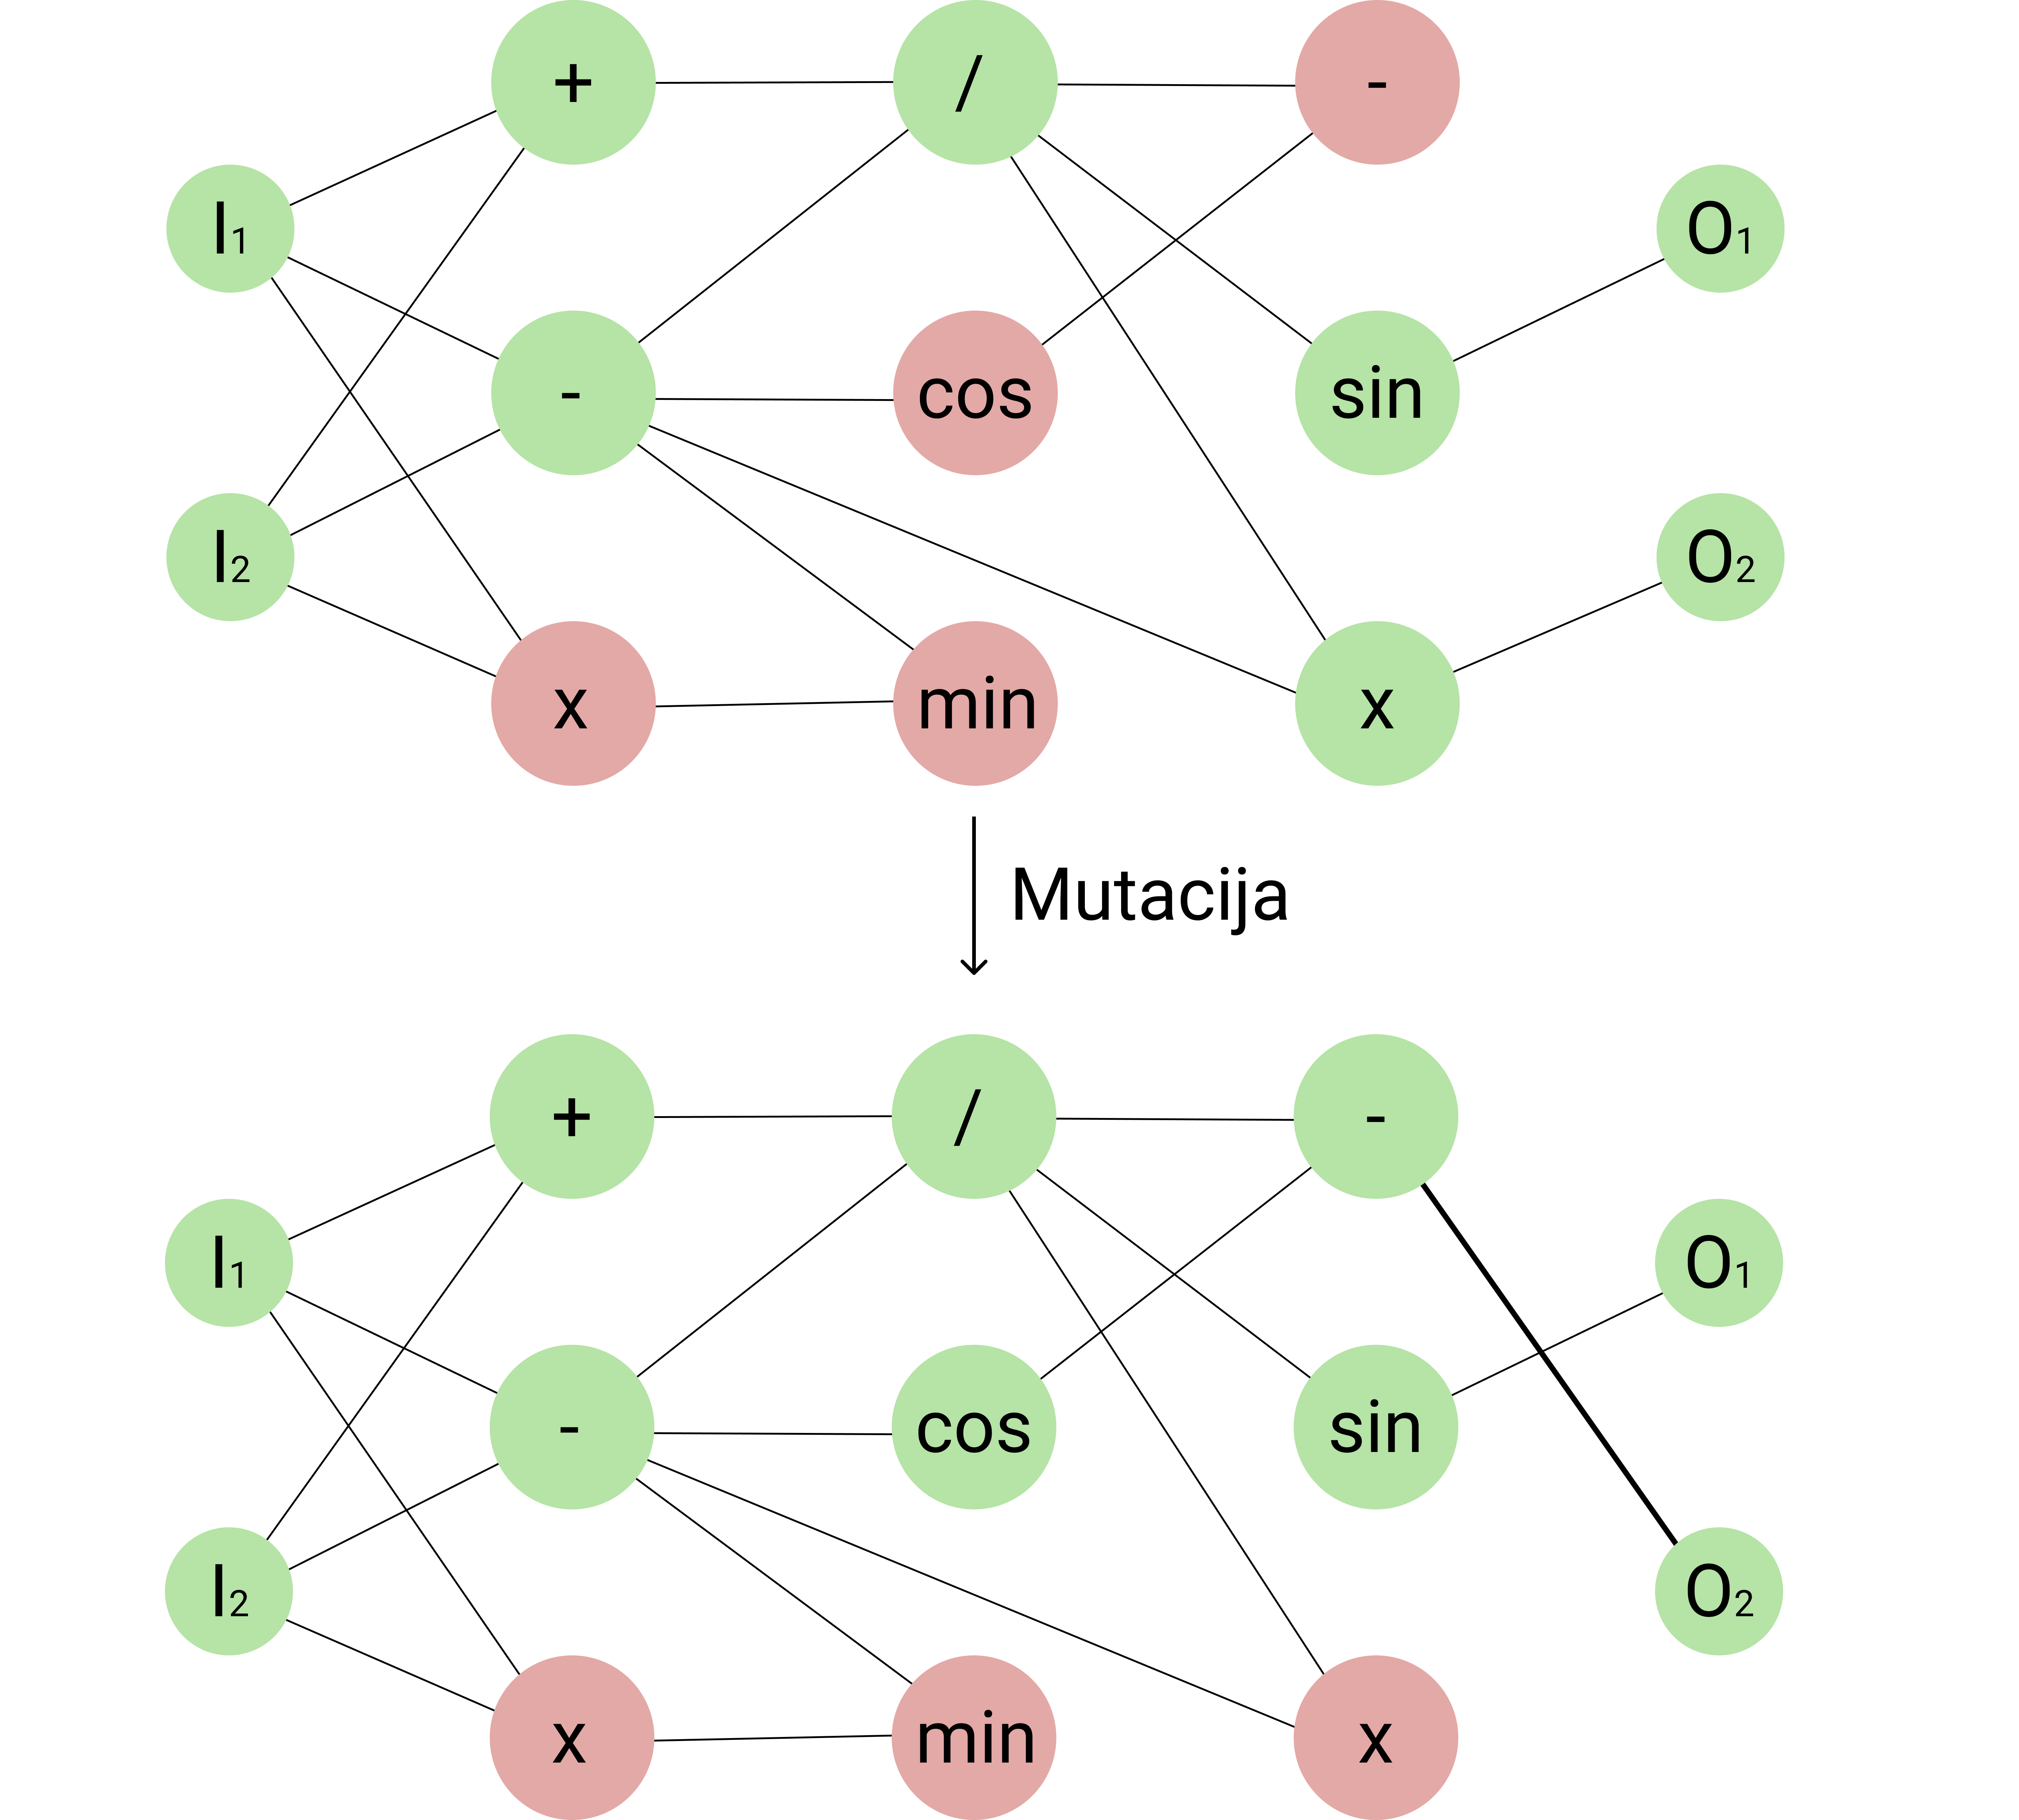
\includegraphics[width=\linewidth]{Illustrations/cgp_mutation.png}
	\caption{CGP fenotip prije i nakon mutacije. Aktivni, odnosno, neaktivni čvorovi jasno su naznačeni kao i novo-nastala veza.}
	\label{fig:cgp_mutation}
\end{figure}

\subsubsection{Križanje}
Kao što je spomenuto, genotip je vektor cijelih brojeva fiksne duljine.
Velika prednost toga je što je križanje iznimno lako za ostvariti.
Za razliku od mutacije, ne moramo paziti na domene pojedinih gena.
Operator križanja koji se koristi je križanje u $k$ točaka gdje je $k = 1$.
Iako je lako izvodivo, sa sobom nosi nedostatke.
Rezultat križanja je spajanje dva podgrafa koja zajedno daju lošije rezultate nego dva originalna CGP-a zasebno.
\cite{cgp_experiment} predstavlja nekolicinu radova s obečavajućim rezultatima koristeći eksperimentalne načine križanja, no istraživanje i isprobavanje istih nije u sklopu ovog rada.

\subsubsection{Algoritam}
Algoritam evolucije koji predlaže \cite{cgp} je $1 + \lambda$.
$\lambda$ može biti proizvoljna vrijednost koja predstavlja broj potomaka nastalih mutacijom.
Spomenuti rad predlaže korištenje $\lambda = 4$.
Rezultati eksperimenata koji će biti prikazani u nastavku potvrđuju tu tvrdnju iako sam mjestimično koristio $\lambda = 8$ kao što predlaže \cite{Sekanina2011}.
Evolucija je detaljnije prikazana algoritmom \ref{alg:cgp_evolution}.

\begin{algorithm}
	\caption{Strategija $1 + \lambda$ za evoluciju CGP-a}
	\label{alg:cgp_evolution}
	\begin{algorithmic}
		\FOR{i unutar $0 \leq i \leq \lambda$}
			\STATE Stvori $CGP_i$
		\ENDFOR
		\STATE Od stvorenih CGP odaberi najbolji i definiraj ga kao roditelja
		\WHILE{uvjet zaustavljanja nije ostvaren}
			\FOR{i unutar $0 \leq i < \lambda$}
				\STATE Mutiraj roditelja i stvori novi $CGP_i$
			\ENDFOR
			\STATE Evaluiraj nove potomke i odaberi najbolji
			\IF{najbolji potomak pokazuje bolje ili jednako ponašanje nego roditelj}
				\STATE Roditelj $\leftarrow$ Najbolji potomak
			\ENDIF
		\ENDWHILE
	\end{algorithmic}
\end{algorithm}



\chapter{Konvolucija slike}
\section{Što je konvolucija}
Konvolucija je u svojoj srži jednostavna matematička operacija koja je prikladna za obradu signala.
U osnovi, fotografija je vrsta signala, a konvolucija je crna kutija koja pretvara jedan signal, odnosno, sliku, u drugi.
Prednost konvolucije je što ne gleda samo jednu vrijednost, već i susjedne vrijednosti, pružajući tako dodatan kontekst.

\section{Jezgra konvolucije (\emph{eng. Kernel})}
Jezgra konvolucije, često nazvana \emph{prozor}, matrica je malih, neparnih dimenzija najčešće $3 \times 3$ ili $5 \times 5$.
Primjer jezgre može biti: 
$$
\begin{bmatrix}
	-1 & 0 & -1 \\
	-1 & 8 & -1 \\
	-1 & 0 & -1
\end{bmatrix}
$$
Jezgrom se prelazi preko željene matrice svim retcima i stupcima izvodeći u svakom koraku množenje po članovima (\cite{conv_pres}), primjerice:

\[
\begin{bmatrix}
	4 & 1 & 5\\
	1 & 2 & 6 \\
	9 & 7 & 3
\end{bmatrix}
\times
\begin{bmatrix}
	-1 & 0 & -1 \\
	-1 & 8 & -1 \\
	-1 & 0 & -1
\end{bmatrix}
=
\begin{bmatrix}
	-4 & 0 & -5\\
	-1 & 16 & -6 \\
	-9 & 0 & -3
\end{bmatrix}
\]
Jezgra konvolucije i sama konvolucija prikladni su za obradu slike iz razloga što računalo sliku i vidi kao dvodimenzionalnu matricu.
Spomenuto je lako zamislivo posebice u slučaju crno-bijele slike gdje vrijednosti mogu biti $\in [0, 255]$, gdje je $0$ crna, a $255$ bijela boja.

\subsection{Rubne vrijednosti}
Problem koji se može javiti jest kako se koristiti rubnim vrijednostima za potrebe korištenja u jezgri.
Na primjer, gornji lijevi rub slike nema susjedne vrijednosti gore i lijevo od sebe.

\paragraph{Produljivanje}
u slučaju nedostatka susjedne vrijednosti na njegovo mjesto samo kopira najbližu postojeću vrijednost (Ilustracija \ref{fig:extend_edge}).

\paragraph{Obgrljivanje}
promatra sliku kao da je beskonačna po veličini, u obje osi.
U slučaju nedostatka vrijednosti  jednostavno dobiva vrijednost sa suprotne strane.
Također, to je metoda koju sam ja koristio u implementaciji i eksperimentima te pruža dobre rezultate (Ilustracija \ref{fig:wrap_edge}).

\paragraph{Preskakivanje}
uopće ne promatra rubne vrijednosti slike te zaobilazi problem nepostojećih rubnih vrijednosti u potpunosti.
Problem koji se može javiti jest da je rezultantna matrica $G$ manja od izvorne matrice $F$.

\begin{figure}
	\caption{Grafički prikaz dva različita načina upravljanja rubnim vrijednostima s označenim rubom slike i trenutnom pozicijom jezgre}
	\begin{subfigure}[t]{0.48\textwidth}
		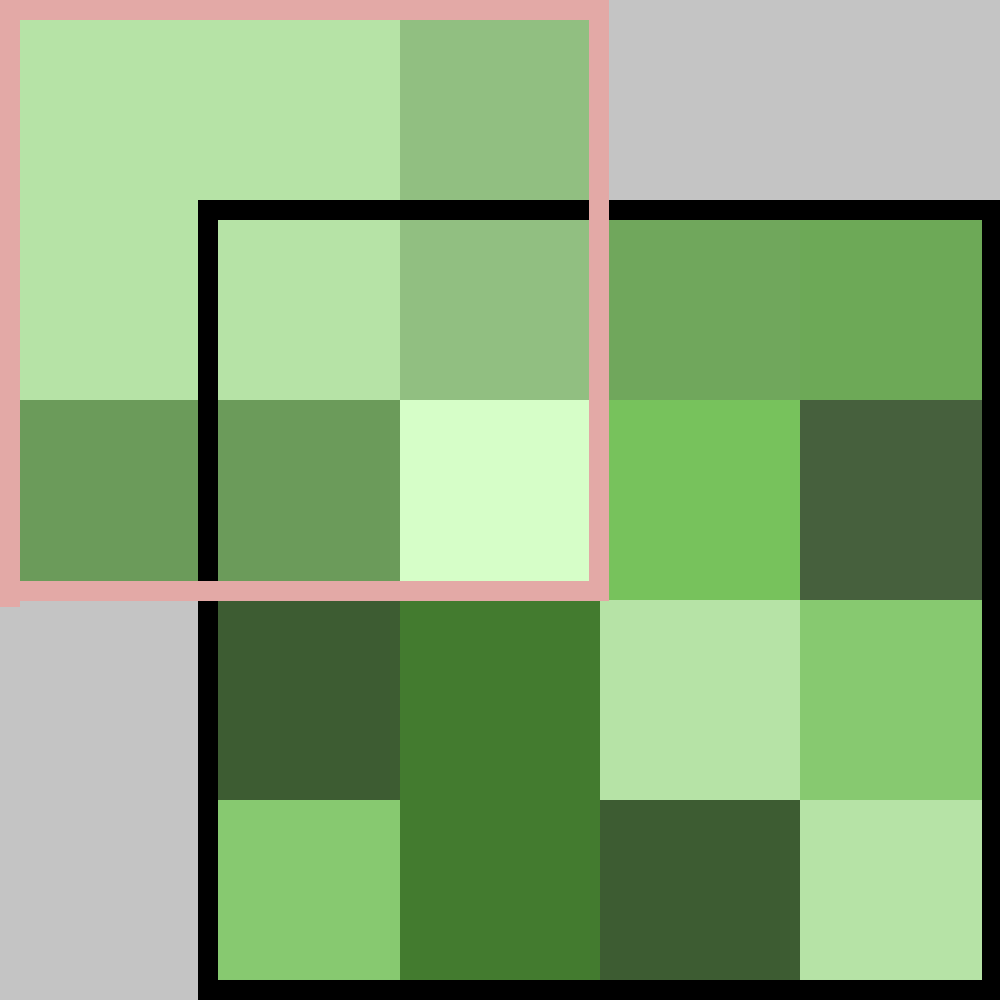
\includegraphics[width=\textwidth]{Illustrations/extend.png}
		\caption{Upravljanje rubom produljivanjem trenutno promatrane jezgre}
		\label{fig:extend_edge}
	\end{subfigure}
	\begin{subfigure}[t]{0.48\textwidth}
		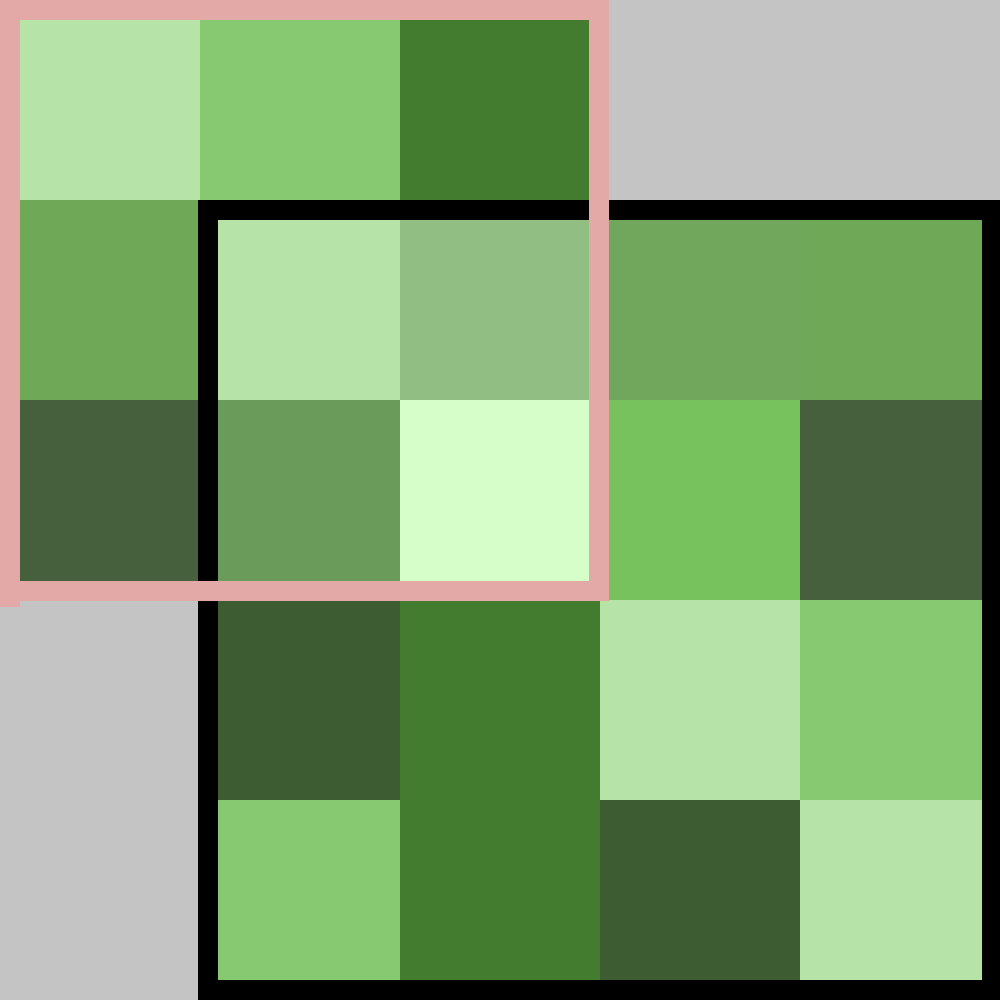
\includegraphics[width=\textwidth]{Illustrations/wrap.png}
		\caption{Upravljanje rubom obgrljivanjem slike}
		\label{fig:wrap_edge}
	\end{subfigure}
\end{figure}

\section{Operacija konvolucije}
Konvolucija se matematički može prikazati kao
$$g(x, y) = \omega \cdot f(x,y) = \sum_{dx=-a}^{a} \sum_{dy=-b}^{b} \omega(dx, dy)\cdot f(x + dx, y + dy)$$
gdje je $g(x,y)$ rezultantna slika, $f(x, y)$ izvorna slika a $\omega$ jezgra.

\section{Provedeni eksperimenti}

\subsection{Micanje šuma}
Prvi problem koji sam definirao je problem rekonstrukcije slike s dodanim šumom.
Promatramo sliku, definiranu kao matrica $I$ veličine $w \times h$ gdje za svaki element $x$ na koordinatama $(i, j)$ vrijedi $x_{(i, j)} \in [0, 255]$ što predstavlja intentzitet boje od crne prema bijeloj. \\
Sintetički šum koji sam dodao vrste \emph{"Salt and pepper"} odnosno soli i papra nazvan je tako jer određeni postotak nasumičnih vrijednosti postavi na bijelu ili crnu boju (slika \ref{fig:salt_pepper_example}).

\begin{figure}
	\centering
	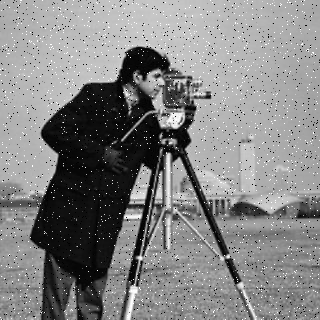
\includegraphics[width=0.5\linewidth]{Experiments/GrainRemoval/input_example.png}
	\caption{Primjerak fotografije s $5\%$ šuma soli i papra}
	\label{fig:salt_pepper_example}
\end{figure}

Postotak slike na koji sam odlučio primjeniti šum je $5\%$, slično kao i \cite{cgp_image_processing} i \cite{Sekanina2011}.
U nastavku rada također ću predstaviti rezultate na većem postotku šuma od $40\%$.

Cilj eksperimenta je evoluirati filter $f(x)$ koristeći konvolucijske metode i CGP koji će od oštećene slike $D$ reproducirati novu $Y = f(D)$ što bližu neoštećenom originalu $I$.
$$
\min_{Y, i, j} |Y_{(i, j)} - I_{(i, j)}|
$$
Iz susjedstva svake vrijednosti želimo dobiti što precizniju promatranu vrijednost. \\
Polazišna pretpostavka je ta su susjedne vrijednosti na slici u međusobnoj korelaciji do određene mjere te mogu pomoći u zaključivanju originalne vrijednosti.
Problem koji se može javiti je da u promatranom susjedstvu također imamo vrijednost koja je šum što narušava pretpostavku korelacije.
Navedeni problem je zanemaren te je CGP-u ostavljeno kao problem koji treba riješiti bez ljudskog znanja.

Jezgra $\omega$ koju sam odlučio koristiti je veličine $3 \times 3$ koja promatra $Moore$-ovo susjedstvo (\cite{jakobovic}).

\[
	\omega_{(i, j)}
	=
	\begin{bmatrix}
		x_{(i - 1, j - 1)} && x_{(i - 1, j)} && x_{(i - 1, j + 1)}\\
		x_{(i, j - 1)} && && x_{(i, j + 1)}\\
		x_{(i + 1, j - 1)} && x_{(i + 1, j)} && x_{(i + 1, j + 1)}
	\end{bmatrix}
\]
Razmišljanje iza korištenja jezgre koja ne koristi središnju, promatranu vrijednost je što tu vrijednost upravo pokušavamo predvidjeti i njena vrijednost, posebice ako je šum ne smije imati utjecaja.
Detaljniji prikaz djelovanja i rezultata mooreove jezgre vidljiv je na ilustraciji \ref{fig:moore_example}

\begin{figure}
	\centering
	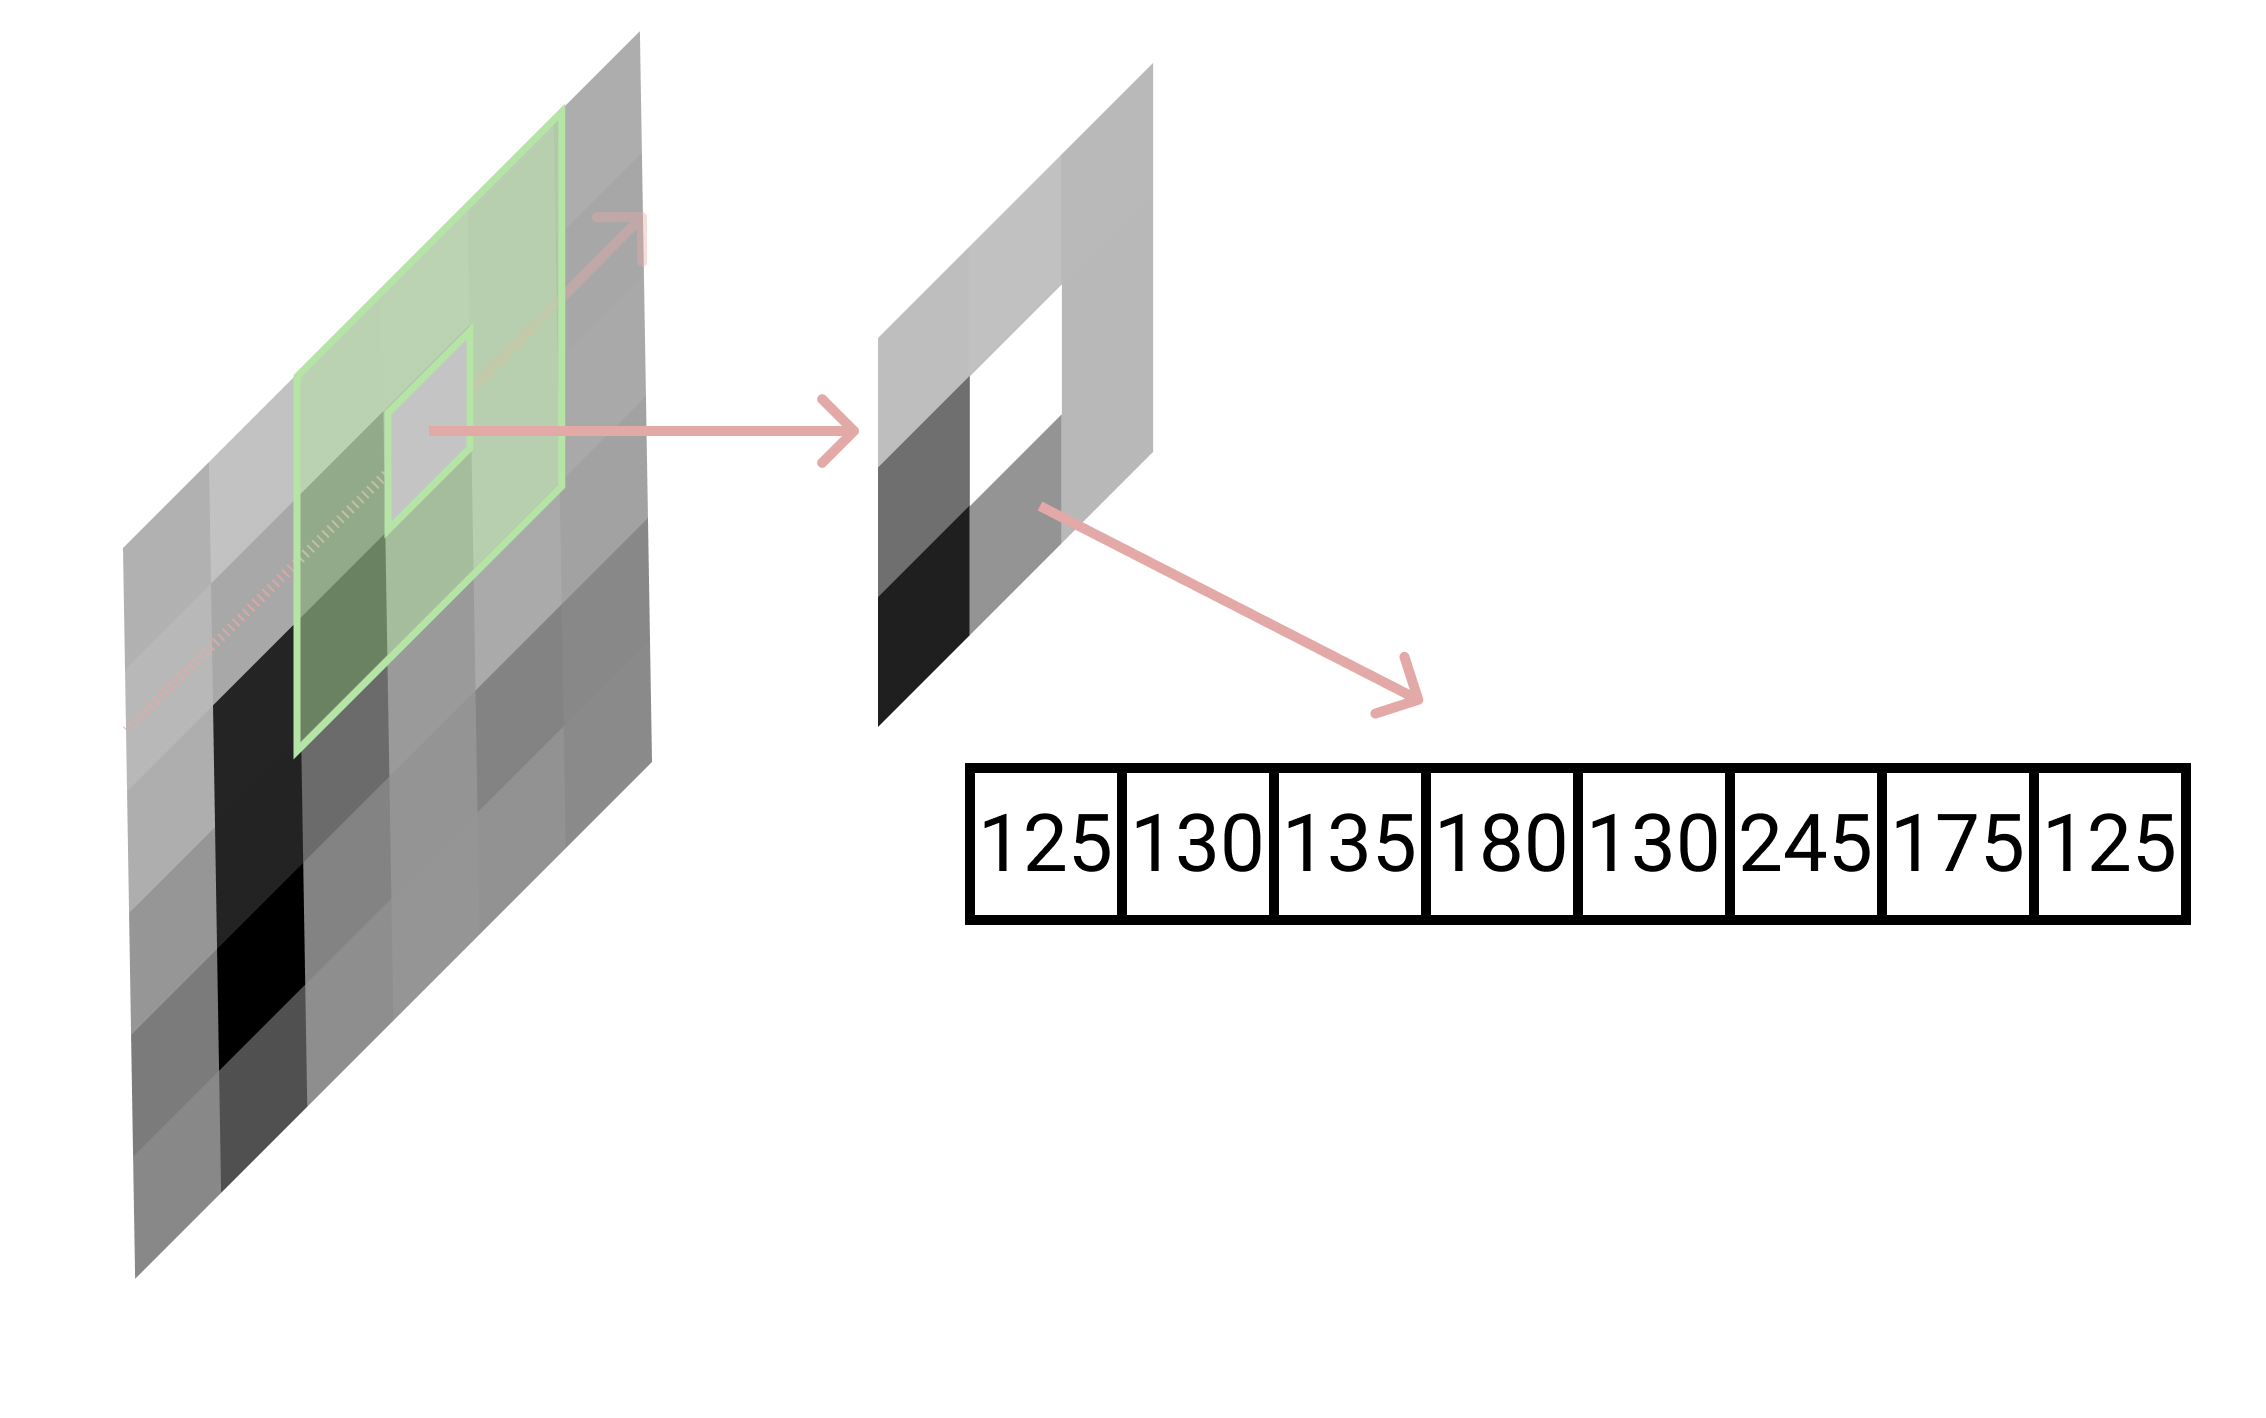
\includegraphics[width=0.8\linewidth]{Illustrations/moore.png}
	\caption{Primjer čitanja slike mooreovom jezgrom te transformacija iz preuzetog dijela slike u vektor vrijednosti koristivih CGP-u}
	\label{fig:moore_example}
\end{figure}



\subsection{Detektiranje rubova (\emph{eng. Edge detection})}
Detektiranje rubova može se promatrati kao tehnika čitanja rubova objekata vidljivih na slici.
Samo po sebi jedna je od osnovnih, nisko razinskih tehnika računalnog vida s mnogim primjenama visoke razine, uključujući detekciju objekata i segmentaciju slike (\emph{eng. Image Segmentation}) (\cite{Liu_2019}).

Problem je definiran kao pokušaj imitiranja rada \emph{Sobel} operatora.

 \paragraph{Sobel operator} također je operator koji koristi konvoluciju.
 Koriste se dvije konvolucijske jezgre (\cite{Sekanina2011}):
 \[
	 p = \frac{1}{8}
	 \begin{bmatrix}
		 -1 && 0 && 1 \\
		 -2 && 0 && 2 \\
		 -1 && 0 && 1
	 \end{bmatrix}
	 ,\ 
	 q = \frac{1}{8}
	 \begin{bmatrix}
		 -1 && -2 && -1 \\
		 0 && 0 && 0 \\
		 1 && 2 && 1
	 \end{bmatrix}
 \]
Zajedno, jezgre služe kako bi se izračunao gradijent slike.
Jezgra $p$ koristi se kako bi se izračunala procjena derivacije za horizontalne promjene, a $q$ za vertikalne. \\
Vrijednost novonastale slike $G$ na koordinatima $(i, j)$ računa se kao
$$
G_{(i, j)} = c + |p_{(i, j)}| + |q_{(i, j)}|
$$
gdje je $c$ proizvoljna konstanta, npr. $c = 128$.
Primjer djelovanja Sobel operatora na fotografiju Lene vidljiv je na slici \ref{fig:lena_sobel}.

\begin{figure}
	\centering
	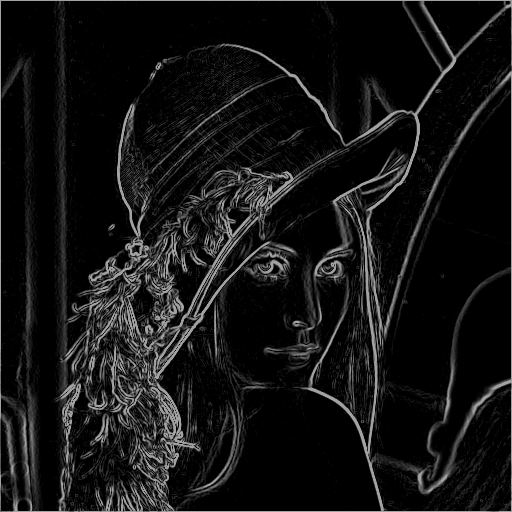
\includegraphics[width=0.6\linewidth]{Experiments/EdgeDetection/lena_sobel.png}
	\caption{Primjer djelovanja Sobel operatora na fotografiju Lene}
	\label{fig:lena_sobel}
\end{figure}

\subsubsection{Postavke}
Za razliku od micanja šuma koristi se konvolucijska jezgra koja prihvaća i srednju promatranu vrijednost.
Time, filter možemo definirati kao $f(x): [0, 255]^9 \rightarrow [0, 255]$.

Fotografije koje su se promatrale u trening i validacijskoj fazi vidljive su na slici \ref{fig:edge_detection_train_val_in}.
Umjesto direktne usporedbe sa Sobel slikama, odlučio sam se na usporedbu sa slikama dobivenim \emph{Canny} algoritmom.
Slike nastale primjenom Canny algoritma imaju vrijednosti $0$ ili $1$ ovisno pripada li promatrana vrijednost na koordinatama $(i, j)$ rubu što sam koristio kao prednost u razvoju modela.
Jednako kao u više-kategoričkoj klasifikaciji gdje se koristi vektor vrijednosti gdje su sve vrijednosti $0$ osim točne koja je $1$ (\emph{eng. One Hot Encoding}).

\begin{figure}
	\centering
	\caption{Fotografije Lene i Kamermana nakon primjene detekcije ruba \emph{Canny} algoritmom}
	\begin{subfigure}[t]{0.45\textwidth}
		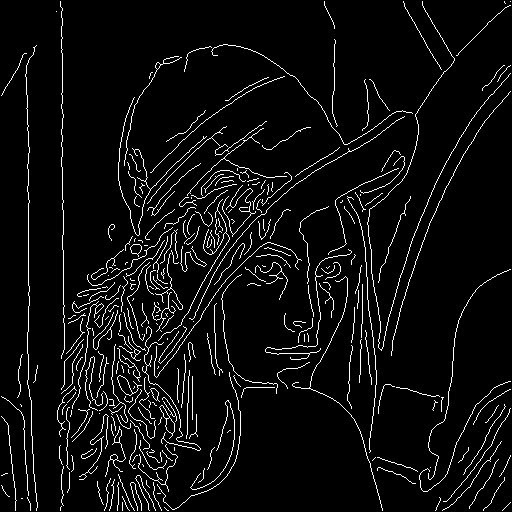
\includegraphics[width=\textwidth]{Experiments/EdgeDetection/lena_canny.jpg}
		\caption{Lena nakon primjene Canny filtera}
		\label{fig:lena_canny}
	\end{subfigure}
	\begin{subfigure}[t]{0.45\textwidth}
		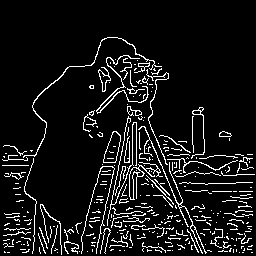
\includegraphics[width=\textwidth]{Experiments/EdgeDetection/cameraman_canny.jpg}
		\caption{Kamerman nakon primjene Canny filtera}
		\label{fig:camerman_canny}
	\end{subfigure}
	\label{fig:edge_detection_train_val_in}
\end{figure}

Problem koji se rano javio je što je $\approx 70\%$ slike vrijednosti $0$, odnosno, crno.
Rezultat toga i korištenja $L1$ pogreške je navođenje modela da teži samo predviđanju te vrijednosti.
Korištenje srednje kvadratne pogreške (\emph{eng. Mean Squared Error (MSE)})
$$err = \frac{1}{n}\sum_{i=1}^{n}(y_{cgp} - y_{skup\ podataka})^2$$
pokazalo se dobrim rješenjem.
U slučaju veće razlike npr. predviđanje $1$ na željenu vrijednost $0$ unutar sume rezultiralo bi razlikom od $255^2$, dok bi manje razlike težile ka $0$.

Tablica \ref{table:edge_detection_function_set} prikazuje funkcije koje su se mogle koristiti u čvorovima.
Vrijednosti nisu morale biti unutar skupa $[0, 255]$, a na izlazu bi se prilagodile najbližoj rubnoj vrijednosti u slučaju da izlaz nije unutar skupa.
Također, ako se funkciji $3$, dijeljenju, prosljedi nepodržana vrijednost u nazivnik, funkcija se koristi kao funkcija identiteta, odnosno $f(x, y) = x$.
Algoritam odabira je $1 + \lambda$ s $\lambda = 8$.
Povećanje parametra $\lambda$ zahtjeva smanjenje najvećeg dozvoljenog broja iteracija koji je postavljen na $20$, puno manje nego pri micanju šuma gdje je definirano kao $500$.

\begin{table}
	\centering
	\begin{tabular}{||c c c c||}
		\hline
		Adresa funkcije & Funkcija & Broj ulaza & Broj izlaza\\ [0.5ex]
		\hline \hline
		0 & $x + y$ & 2 & 1\\
		1 & $x - y$ & 2 & 1\\
		2 & $x \cdot y$ & 2 & 1\\
		3 & $\frac{x}{y}$ & 2 & 1 \\
		4 & $\sqrt{x}$ & 1 & 1\\
		5 & $avg$ & 9 & 1\\
		6 & $min$ & 9 & 1\\
		7 & $max$ & 9 & 1\\
		8 & $\ln(x)$ & 1 & 1\\
		9 & $\sin(x)$ & 1 & 1\\
		10 & $\cos(x)$ & 1 & 1\\
		11 & $step(x)$ & 1 & 1\\ [1ex]
		\hline
	\end{tabular}
	\caption{Funkcije korištene pri detekciji rubova}
	\label{table:edge_detection_function_set}
\end{table}

Promatrani podskupovi veličina su $40 \times 40$.
Time, skup podataka sastoji se od $1600$ vektora ($|v| = 9$), po jedan za svaku promatranu konvolucijsku jezgru.
Trening i validacijski skup uzet je sa iste fotografije Lene u dva odvojena podskupa (\ref{fig:edge_detection_in_out_pair_example}), dok je za testnu fotografiju odabrana fotografija kamermana.

\begin{figure}
	\centering
	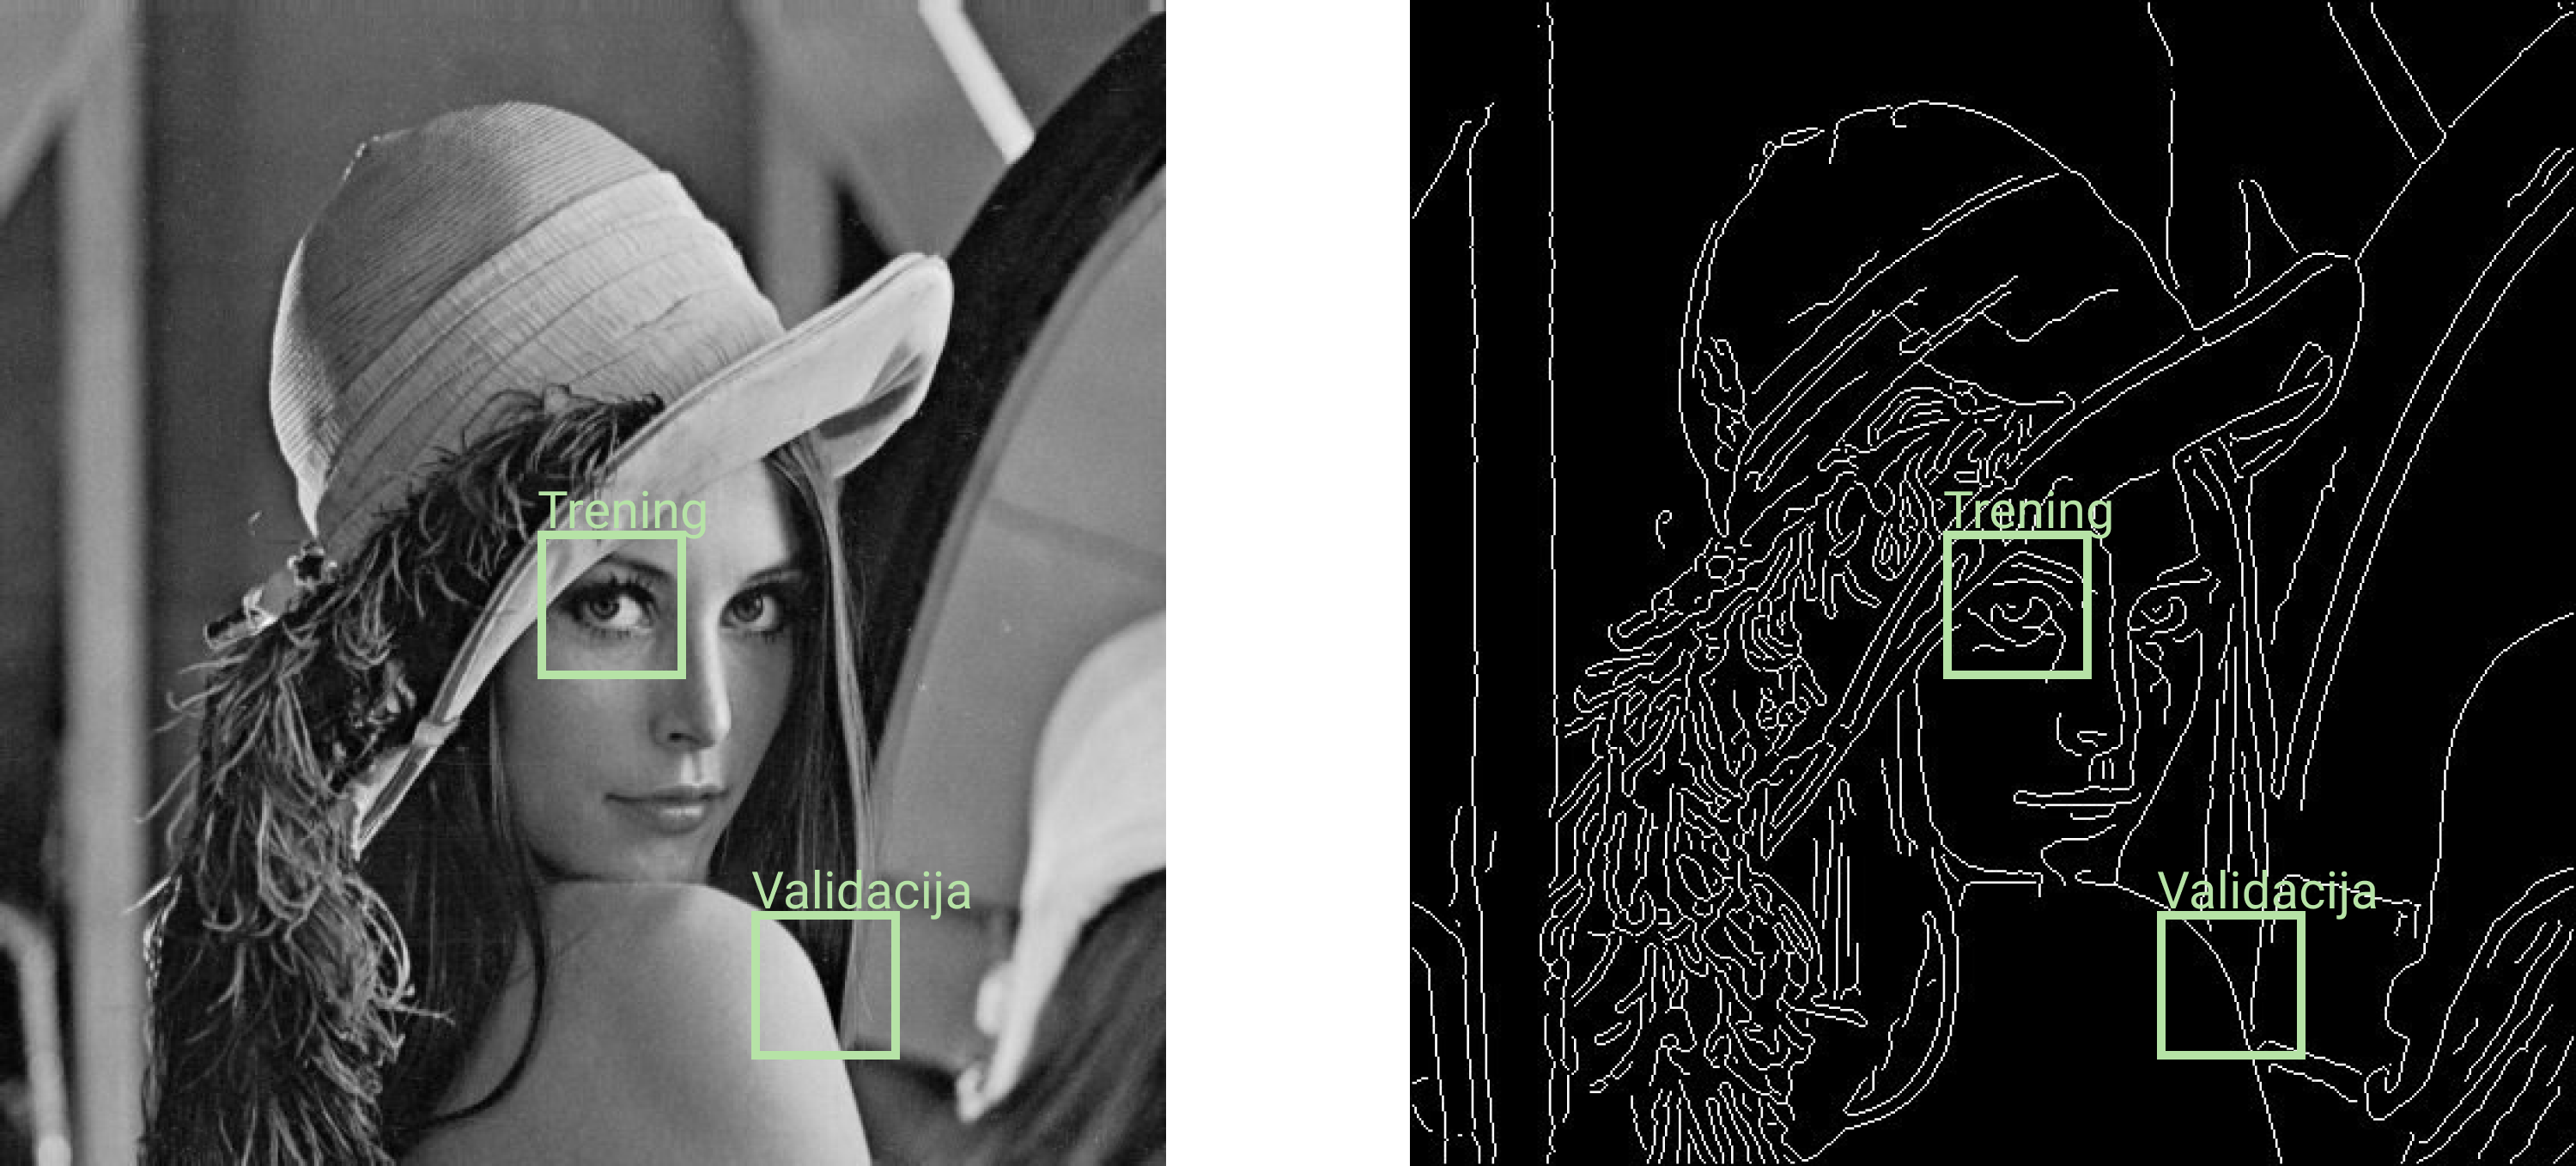
\includegraphics[width=\linewidth]{Experiments/EdgeDetection/edge_detection_in_out_pair.png}
	\caption{Ulazna i željena izlazna slika za detekciju ruba s označenim podskupovima za trening i validaciju}
	\label{fig:edge_detection_in_out_pair_example}
\end{figure}

\subsubsection{Rezultati}
Rezultati detekcije ruba vidljivi su na slikama \ref{fig:edge_detection_results}. % TODO: Dodati graf!
Pomalo neočekivano, rezultati izgledaju bolje na testnoj slici, no to pridodajem značajkama fotografije pogodnijim za detekciju rubova.
Zbog toga, vjerujem da je dosta težak zadatak za detekciju rubova fotografija s vidljivom kosom ili bilo kakvim sitnim detaljima.
Veliku ulogu igrao je i izbor podskupa iz kojeg se isčitavaju podaci za trening.
Količina praznog dijela, vrsta i broj vidljivih krivulja, zajedno s ispravnim odabirom funkcije koju minimiziramo igra najveću ulogu.
U usporedbi s problemom micanja šuma, detekcija rubova rješenje pronalazi iznimno brzo.
Svako pokretanje koje je završilo s uspješnim pronalaskom rješenja konvergiralo je u $\leq 10$ iteracija.

\begin{figure}
	\centering
	\caption{Fotografije Lene i Kamermana prije i nakon detekcije rubova}
	\begin{subfigure}[t]{0.48\textwidth}
		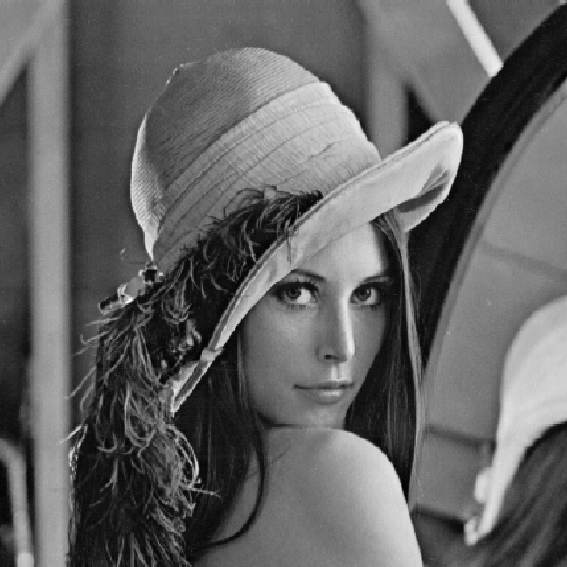
\includegraphics[width=\textwidth]{Experiments/GrainRemoval/lena.png}
	\end{subfigure}
	\begin{subfigure}[t]{0.48\textwidth}
		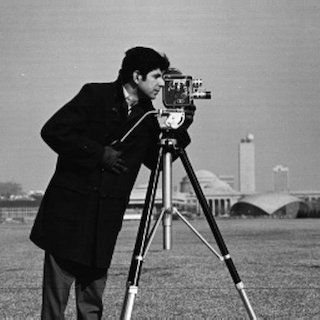
\includegraphics[width=\textwidth]{Experiments/GrainRemoval/cameraman.jpg}
	\end{subfigure}
	\begin{subfigure}[t]{0.48\textwidth}
		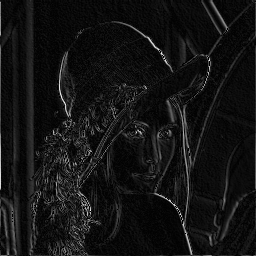
\includegraphics[width=\textwidth]{Experiments/EdgeDetection/lena_edges.png}
	\end{subfigure}
	\begin{subfigure}[t]{0.48\textwidth}
		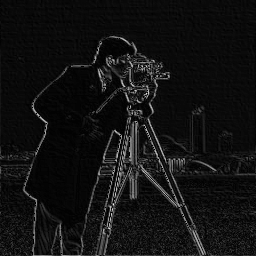
\includegraphics[width=\textwidth]{Experiments/EdgeDetection/camerman_edges.png}
	\end{subfigure}
	\label{fig:edge_detection_results}
\end{figure}

Graf \ref{fig:edge_detection_graph} pokazuje kretanje pogreške na trening i validacijskom skupu podataka.
Greška se čini niska već pri pokretanju no to je zbog prirode algoritma.
Iz početnog stvaranja potencijalnog roditelja kao najbolji odabire se najčešće onaj koji veliku večinu rezultata računa kao $0$ što je u svakom slučaju točno za većinu skupa podataka.
Daljni koraci vrlo brzo konvergiraju točnijim rješenjima.

\begin{figure}
	\centering
	\caption{\emph{MSE} pogreška na trening i validacijskom skupu kroz iteracije algoritma}
	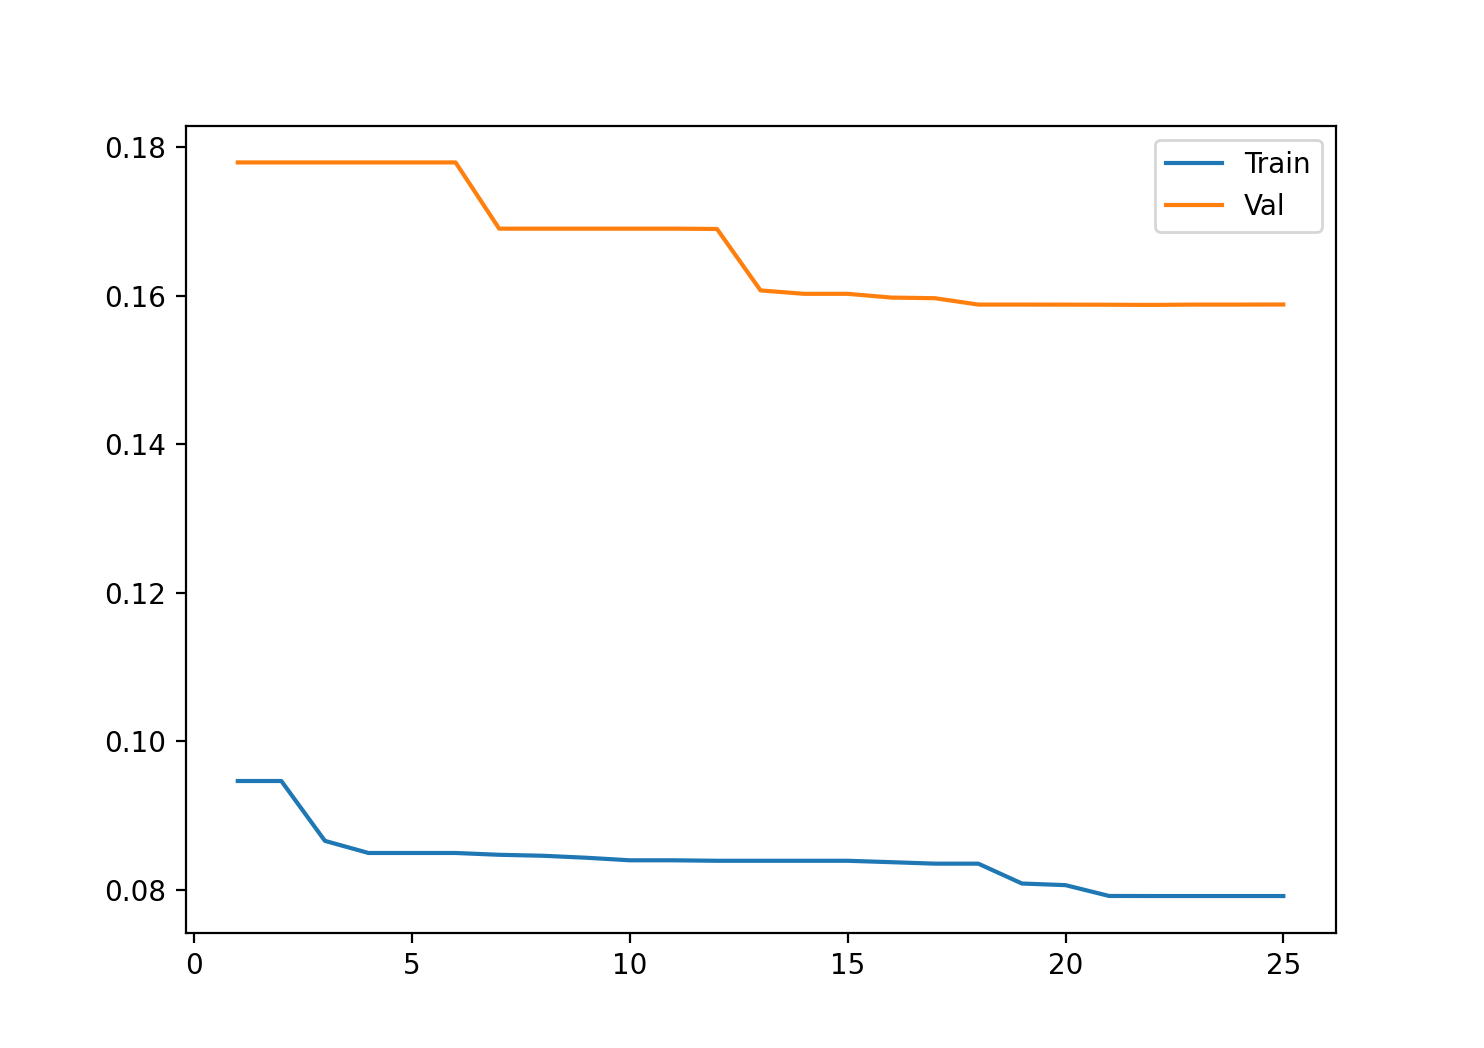
\includegraphics[width=0.6\linewidth]{Experiments/EdgeDetection/edge_detection_graph.png}
	\label{fig:edge_detection_graph}
\end{figure}

Tablica \ref{table:edge_detection_function_quality} prikazuje korisnost pojedinih funkcija.
Kao i u slučaju micanja šuma, svako mjerenje izvršeno je 10 puta te je uzet medijan kao vrijednost za izračun.
Vidljivo je da u ovom slučaju funkcije $step$, $sin$, $cos$ i $min$ ne doprinose radu algoritma, dok su se na primjer $ln$ i $avg$ pokazali važnim.
Zanimljiva je i usporedba funkcija $max$ i $min$ gdje je jedna doprinjela, a druga odmogla radu algoritma.

\begin{table}
	\centering
	\begin{tabular}{||c c||}
		\hline
		Izbačena funkcija & Utjecaj na pogrešku (manje je bolje)\\ [0.5ex]
		\hline \hline
		$step$ & $0.9065$\\
		$sin$ & $0.9100$\\
		$cos$ & $0.9685$\\
		$min$ & $0.9971$\\
		$\bm{osnova}$ & $\bm{1.0}$\\
		$x + y$ & $1.0063$\\
		$x \dot y$ & $1.0619$\\
		$x - y$ & $1.0711$\\
		$\frac{x}{y}$ & $1.2017$\\
		$max$ & $1.3360$\\
		$\sqrt{x}$ & $1.5425$\\
		$ln(x)$ & $1.5605$\\
		$avg$ & $1.5821$\\ [1ex]
		\hline
	\end{tabular}
	\caption{Analiza doprinosa pojedinih funkcija pri detekciji rubova. Osnovno mjerenje dozvoljava sve funkcije iz skupa.}
	\label{table:edge_detection_function_quality}
\end{table}



\chapter{Zaključak}
Zaključak.

\bibliographystyle{fer}
\bibliography{literatura}

\begin{sazetak}
Sažetak na hrvatskom jeziku.

\kljucnerijeci{Ključne riječi, odvojene zarezima.}
\end{sazetak}

% TODO: Navedite naslov na engleskom jeziku.
\engtitle{Cartesian Genetic Programming for image convolution}
\begin{abstract}
Abstract.

\keywords{Keywords.}
\end{abstract}

\end{document}
